\chapter{ESP32 Based Applications}
\section{UGV (Unmanned Ground Vehicle)}
\subsection{Navigation using Fly-sky Transmitter and Receiver} 
\subsubsection{Required components/Software tools}
\begin{itemize}
    \item  UGV chassis with DC motors
    \item  ESP32 micro-controller with Type-B USB cable
    \item  L293D Motor Driver IC
    \item  Fly-sky Transmitter and Receiver
    \item  Breadboard
    \item  Jumper Wires
    \item  Arduino IDE installed on system
\end{itemize}

\subsubsection{Steps}
\begin{itemize}
    \item Make the connections as per the wiring diagram (Figure \ref{Wiring_UGV_flysky1}).
    \item Go to Arduino IDE and write the following program available on the code link at \ref{Code_link_UGV_flysky}.
    \item Compile and upload the program to ESP32 micro-controller using the Type-C programmable cable. Test whether the UGV is navigating as per the command sent from the transmitter.
\end{itemize}

\subsubsection{Code link} \label{Code_link_UGV_flysky}
\begin{tcolorbox}
\url{https://github.com/sachinomdubey/Projects/tree/main/Autonomous\%20Navigation/UGV/ESP32/IDE/UGV_navigation_using_Flyskly/Codes}
\end{tcolorbox}

\begin{figure}[h!]
\centering
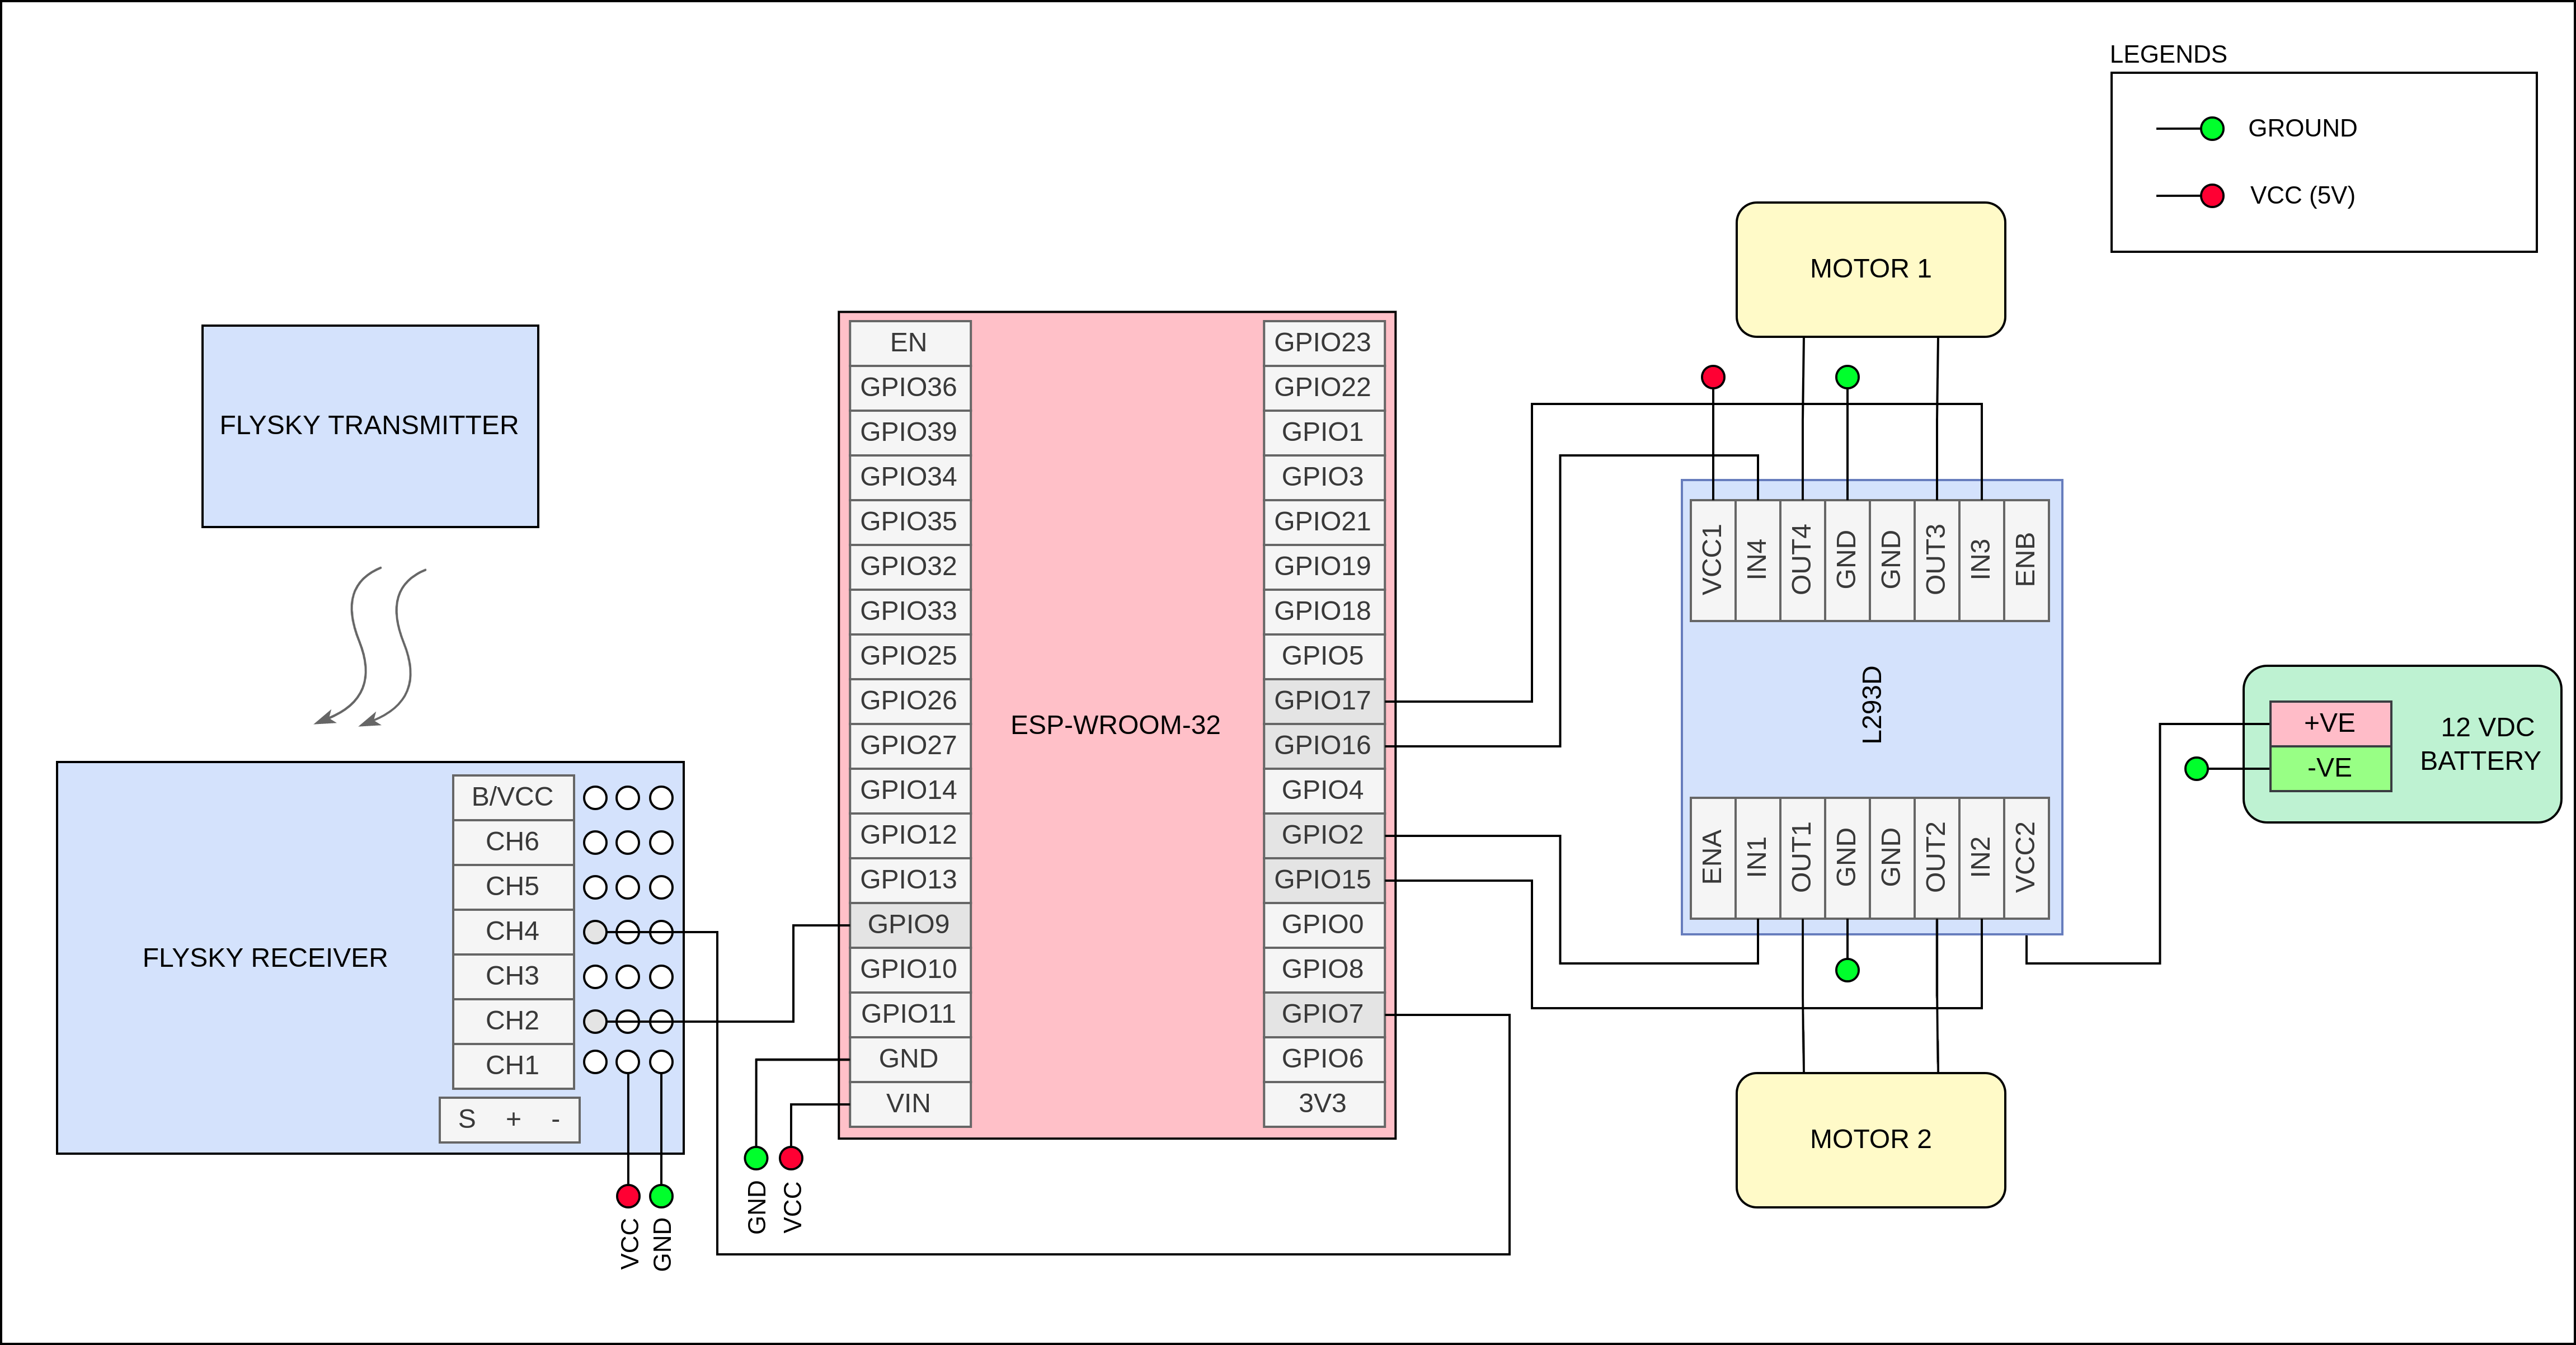
\includegraphics[width=\columnwidth]{./Figures/Wiring_UGV_flysky1.png}
\caption{Wiring Diagram for UGV Navigation using Fly-sky transmitter \& receiver (ESP32)}
\label{Wiring_UGV_flysky1}
\end{figure}

\begin{figure}[h!]
\centering
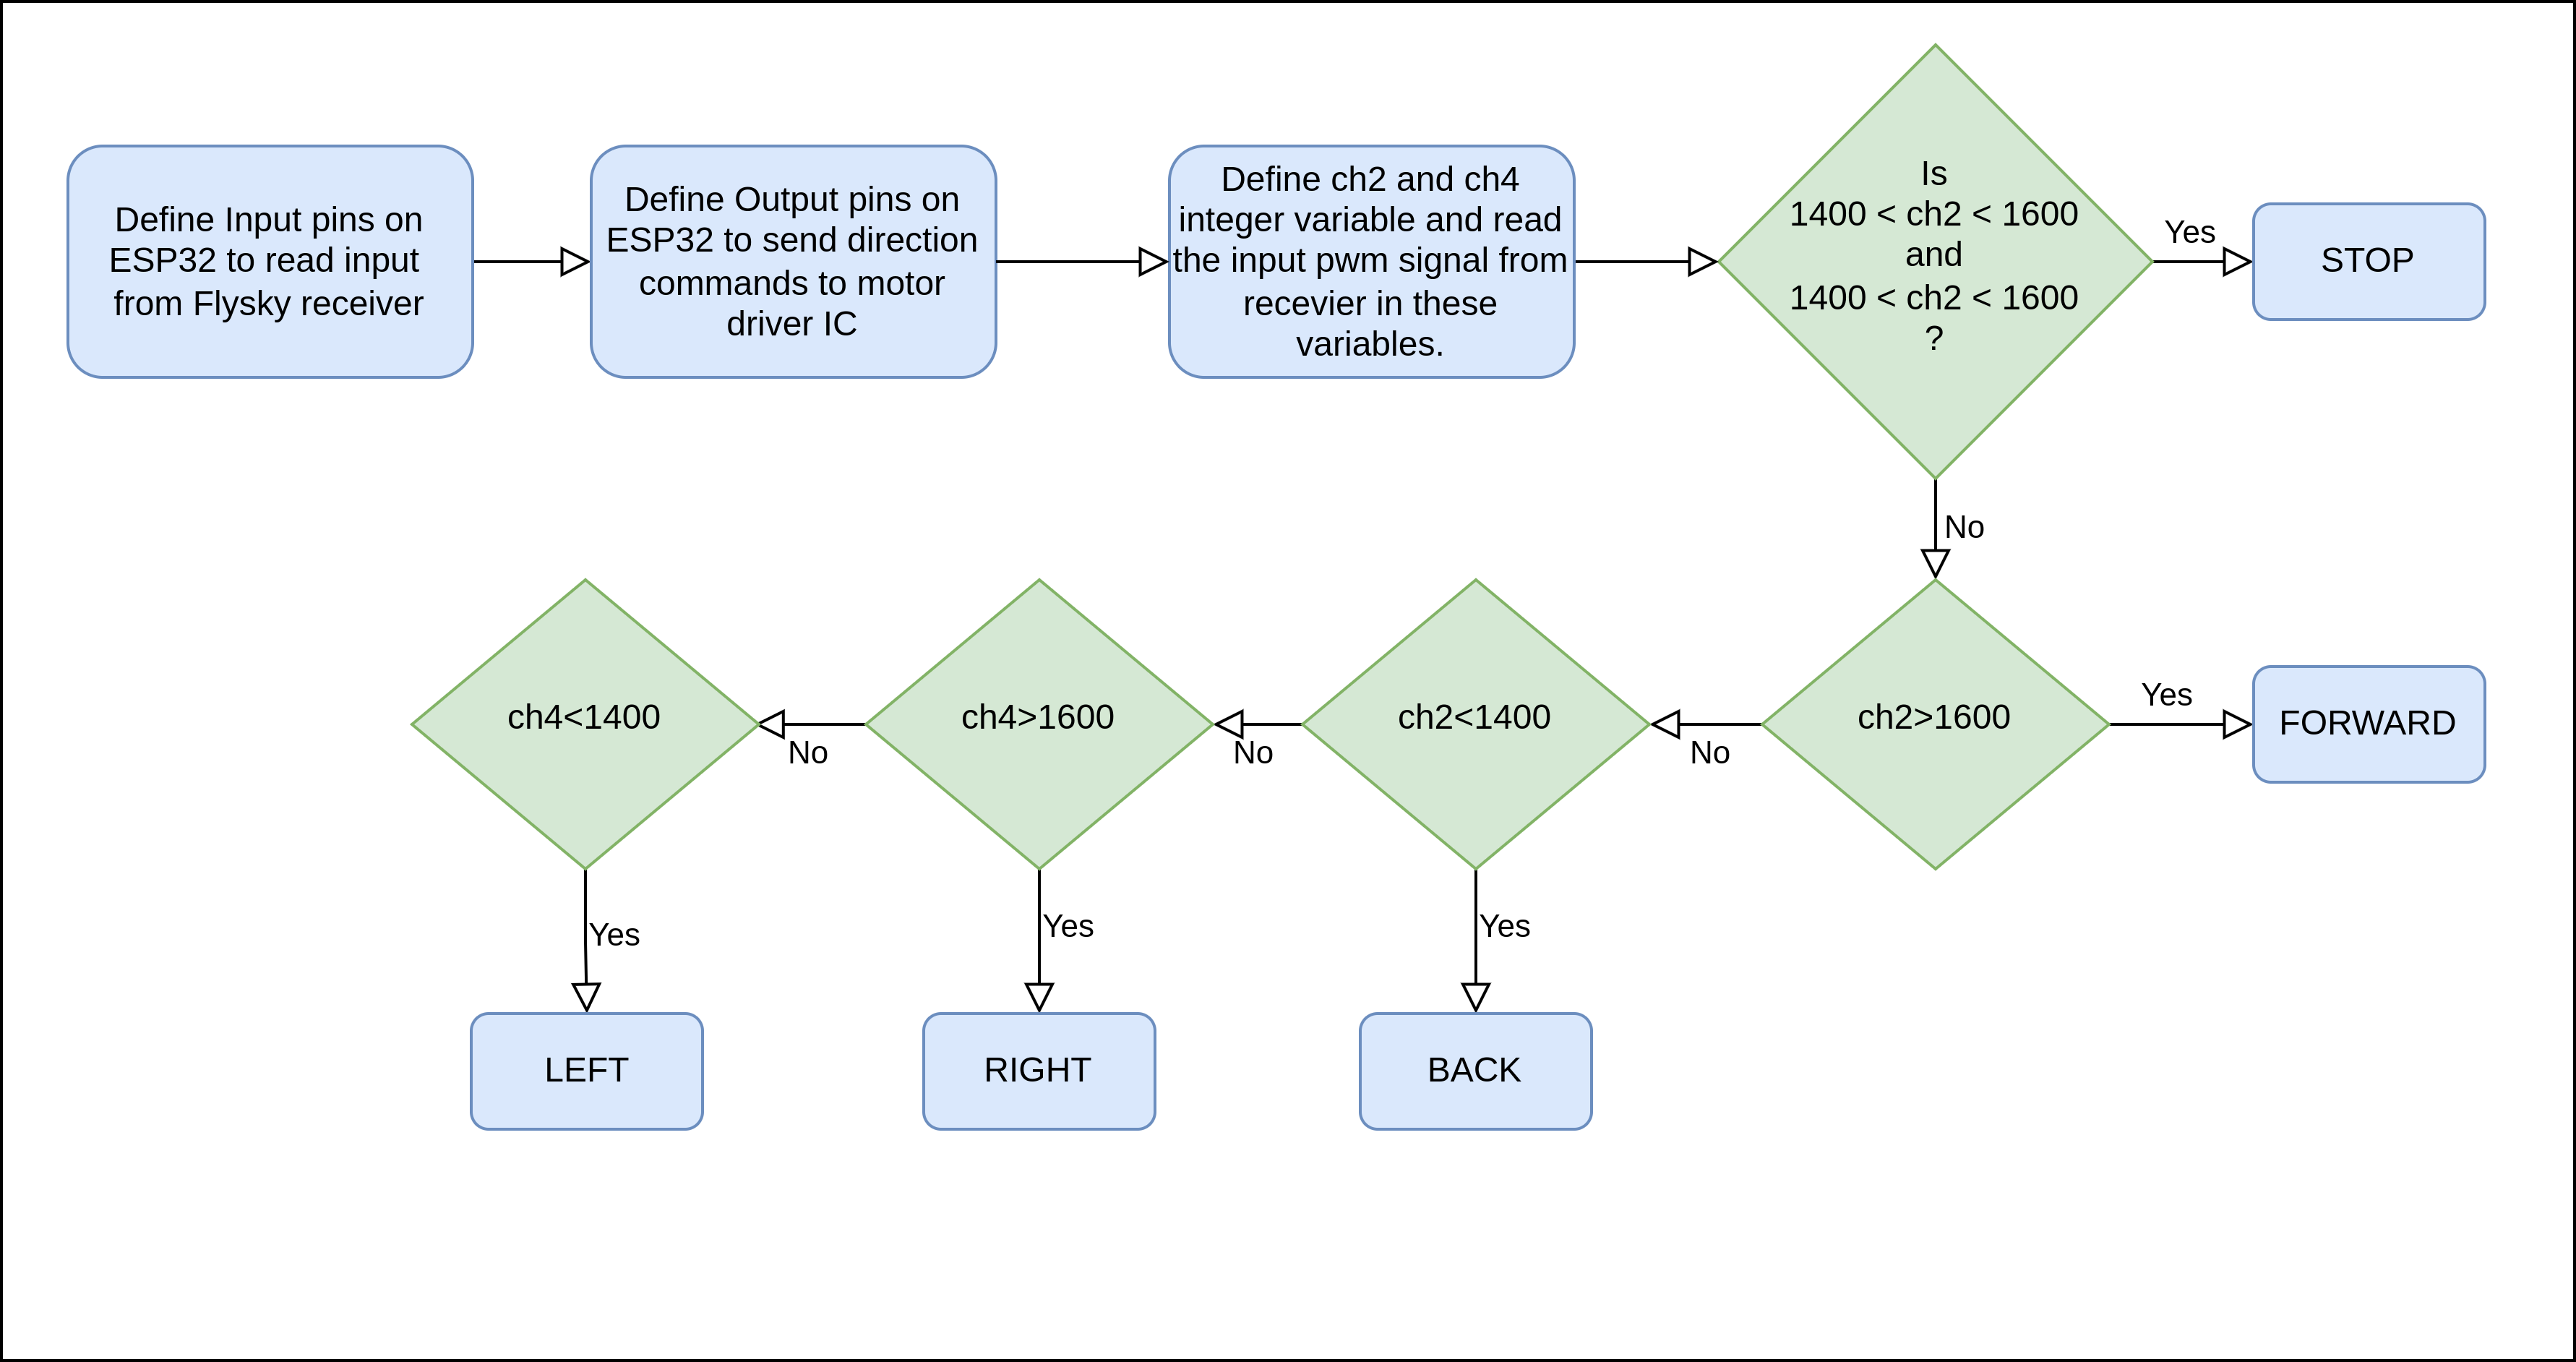
\includegraphics[width=\columnwidth]{./Figures/Flow_UGV_flysky.png}
\caption{Flow Diagram for UGV Navigation using Fly-sky transmitter \& receiver}
\label{Flow_UGV_flysky}
\end{figure}

\subsubsection{Working}
\begin{itemize}
    \item User first give navigation input using the Throttle and Roll sticks on transmitter. This input is transmitted to the receiver wirelessly.
    \item Receiver generates PWM signals on channel-2 and channel-4 as per the navigation input received from the transmitter.
    \item These PWM signals are read by the ESP32 using pulseIn function.
    \item Depending on the read values the program sends suitable commands (forward, backward, left, right and stop) to the direction control pins of Motor driver IC.
\end{itemize}

\subsection{Navigation using Android phone} 
\subsubsection{Required components/Software tools}
\begin{itemize}
    \item  UGV chassis with DC motors
    \item  ESP32 micro-controller with Type-B USB cable
    \item  L293D Motor Driver IC
    \item  Breadboard
    \item  Jumper Wires
    \item  PlatformIO installed on VS code 
    \item  Android phone with Dabble app installed.
\end{itemize}


\subsubsection{Steps}
\begin{itemize}
    \item Make the connections as per the wiring diagram (Figure \ref{Wiring_UGV_phone}).
    \item Go to PlatformIO and execute the "main.cpp" file given at code link at \ref{Code_link_UGV_phone}.
    \item Flash firmware.bin obtained upon execution of the above code to the ESP32. 
    \item Test whether the UGV is navigating as per the command sent from the dabble app installed on Android phone.
\end{itemize}

\subsubsection{{Code link}}\label{Code_link_UGV_phone}
\begin{tcolorbox}
\url{https://github.com/sachinomdubey/Projects/tree/main/Autonomous\%20Navigation/UGV/ESP32/IDE/UGV_navigation_using_android_phone/Codes}
\end{tcolorbox}

\begin{figure}[h!]
\centering
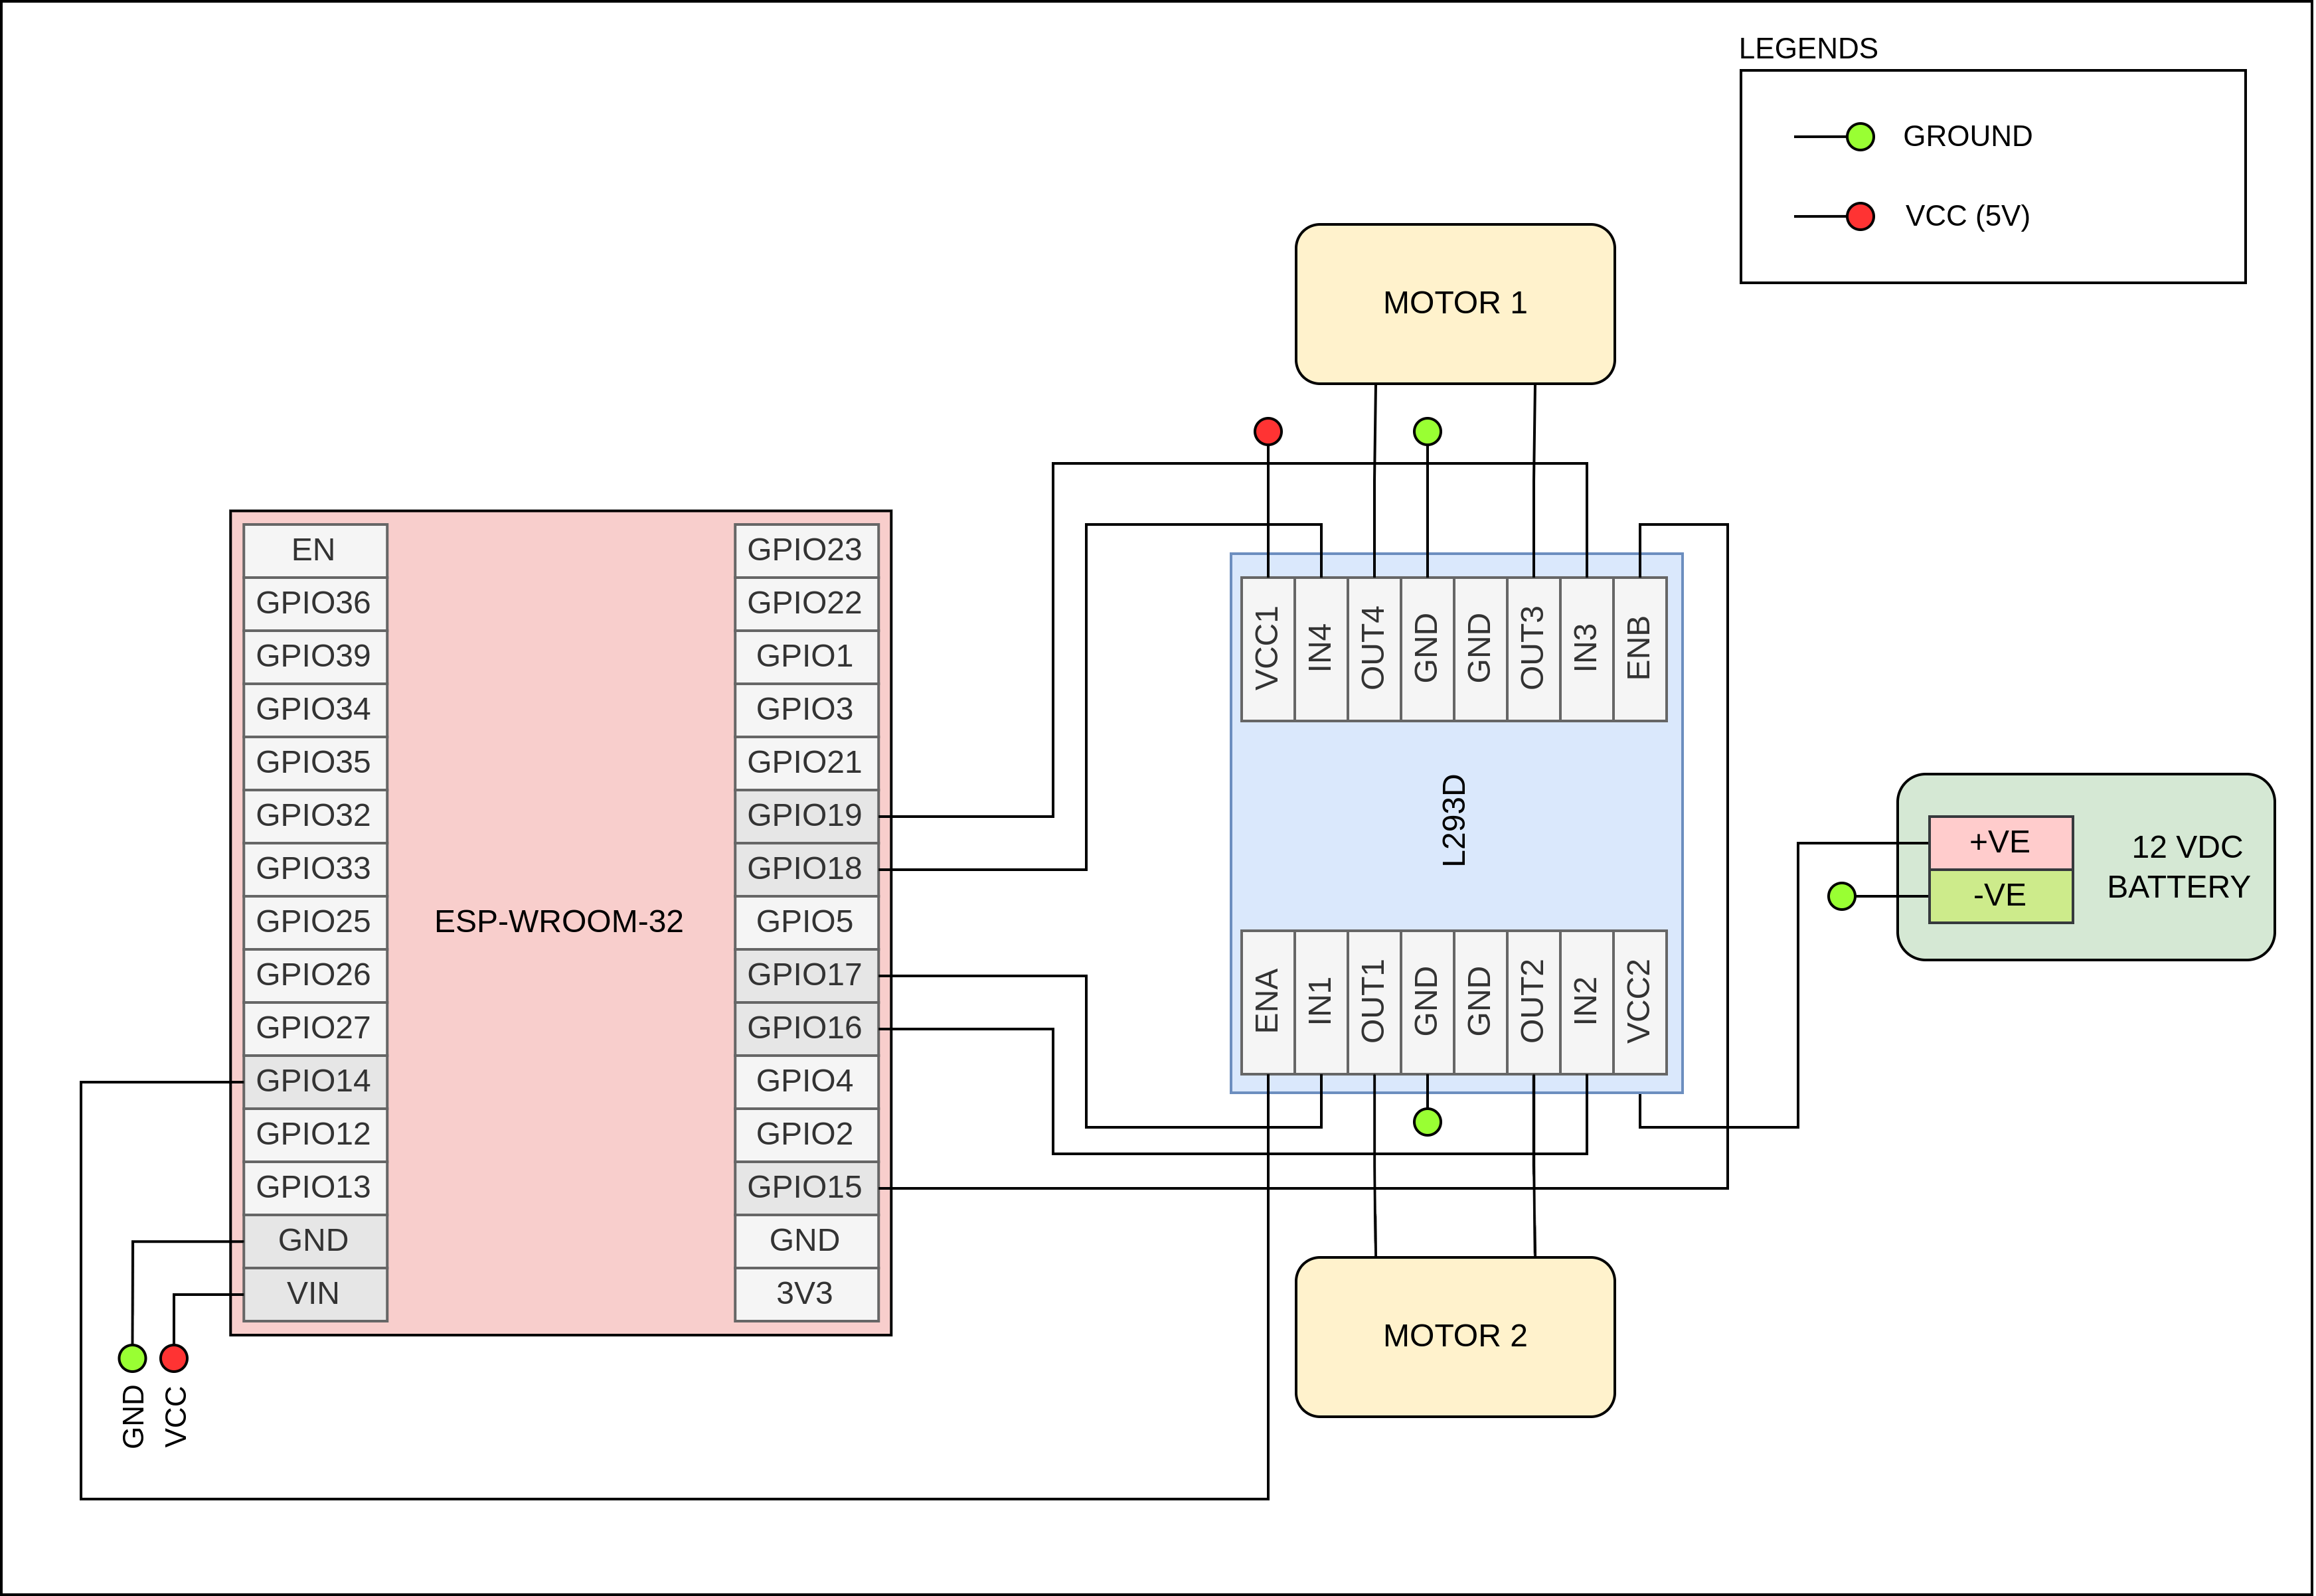
\includegraphics[width=\columnwidth]{./Figures/Wiring_UGV_phone.png}
\caption{Wiring Diagram for UGV Navigation using Android phone (ESP32)}
\label{Wiring_UGV_phone}
\end{figure}

\begin{figure}[h!]
\centering
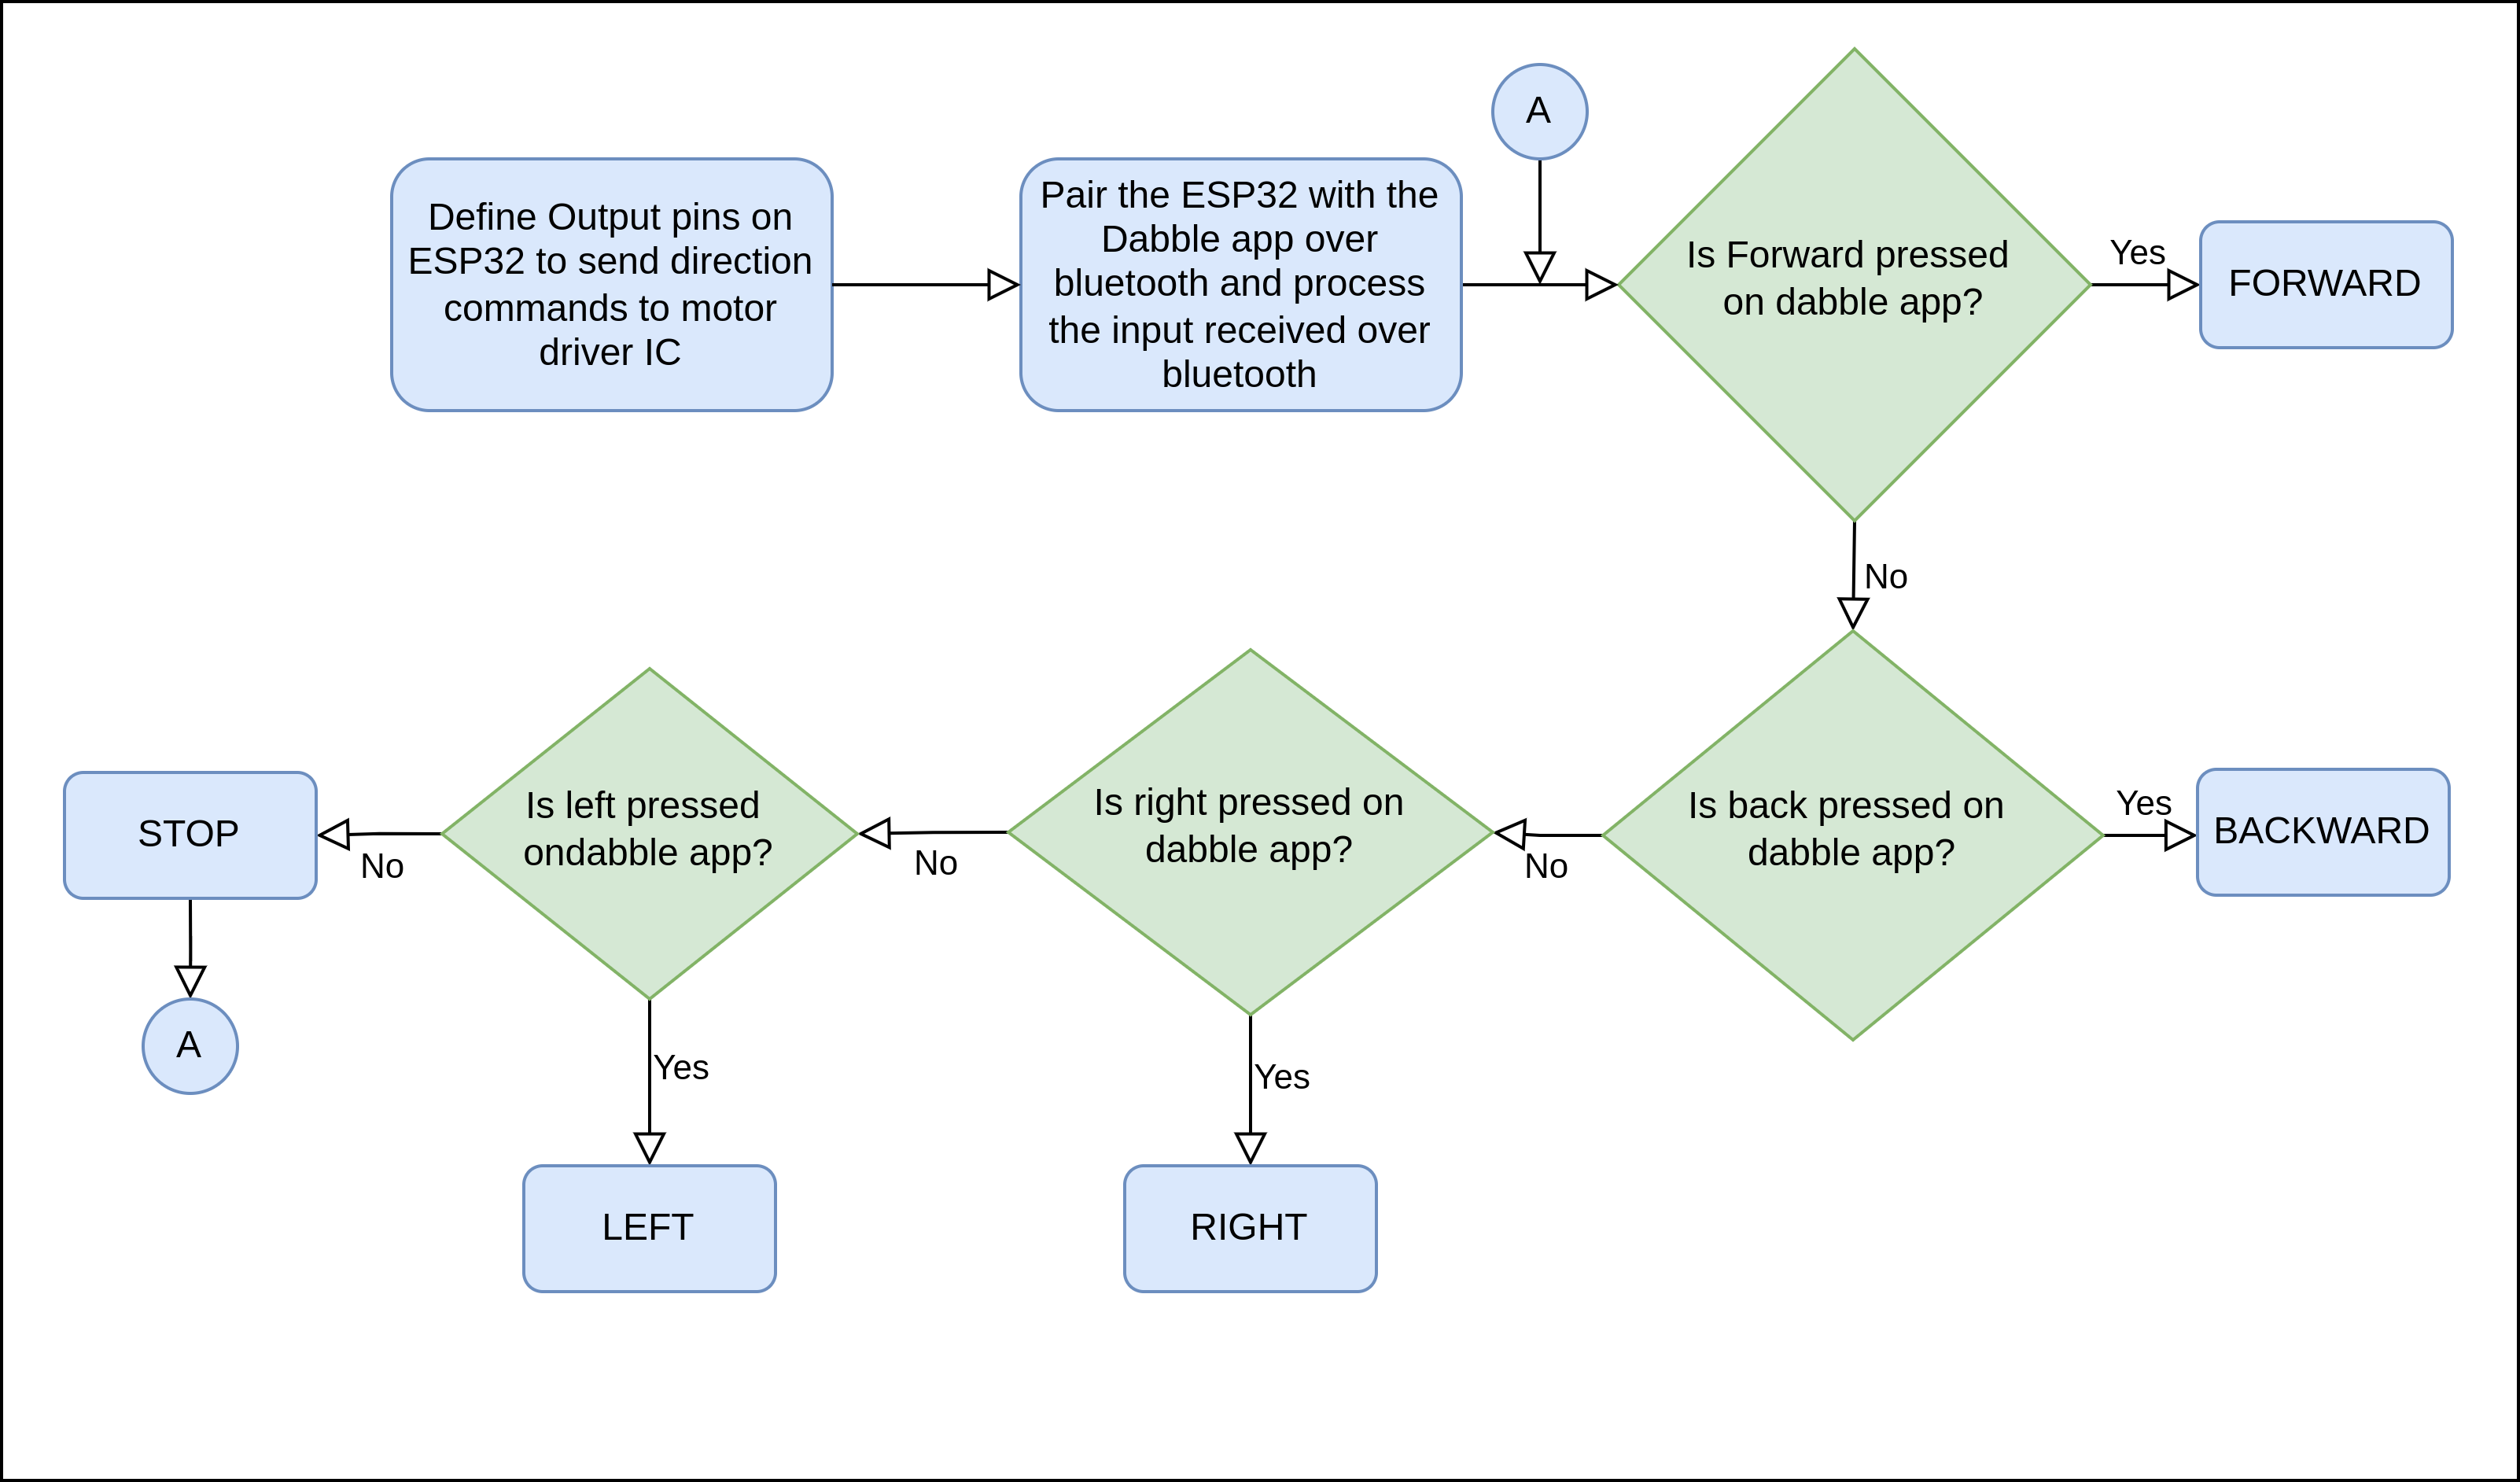
\includegraphics[width=\columnwidth]{./Figures/Flow_UGV_phone.png}
\caption{Flow Diagram for UGV Navigation using Android phone}
\label{Flow_UGV_flysky}
\end{figure}

\subsubsection{Working}
\begin{itemize}
    \item User gives navigation input using the dabble app installed on the android device. The dabble app communicates to ESP32 over bluetooth. The dabble app UI is as shown in figure \ref{Dabble_app_UI}.
    
    \begin{figure}[h!]
    \centering
    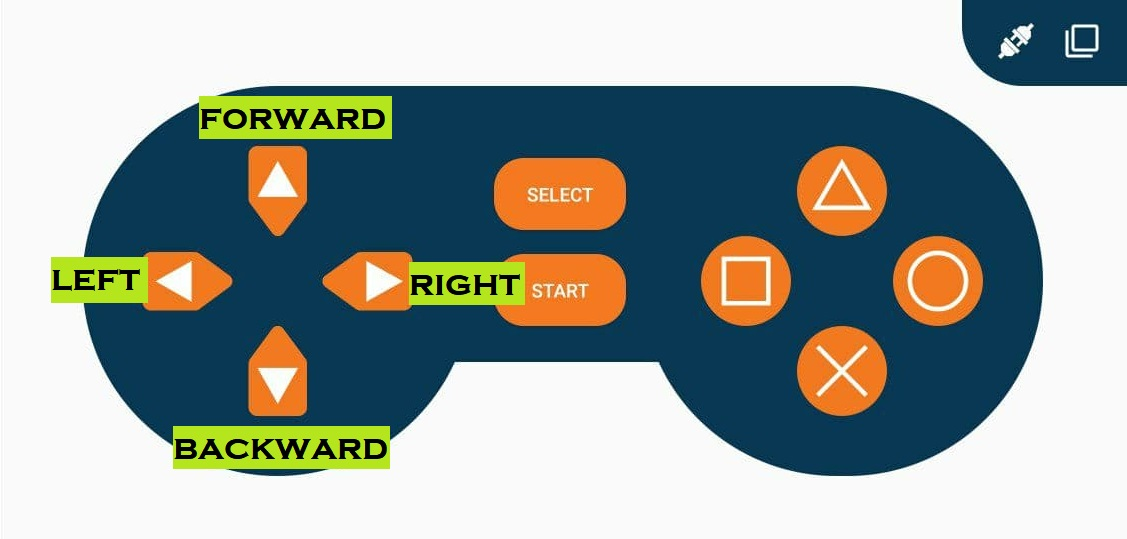
\includegraphics[width=12cm]{./Figures/Dabble_app_UI.jpg}
    \caption{Dabble app user interface}
    \label{Dabble_app_UI}
    \end{figure}
    
    \item Depending on the input received over bluetooth, the program sends suitable commands (forward, backward, left, right and stop) to the direction control pins of Motor driver IC.
\end{itemize}

\clearpage
\newpage
\subsection{Navigation using Speech commands} 
\subsubsection{Required components/Software tools}
\begin{itemize}
    \item  UGV chassis with DC motors
    \item  ESP32 micro-controller with Type-B USB cable
    \item  L293D Motor Driver IC
    \item  Breadboard
    \item  Jumper Wires
    \item  Arduino IDE installed on system
    \item Android Phone
\end{itemize}

\subsubsection{Steps}
\begin{itemize}
    \item Make the connections as per the wiring diagram (Figure \ref{Wiring_UGV_speech}).
    \item Go to Arduino IDE and write the following program available on the code link at \ref{Code_link_UGV_speech}.
    \item Compile and upload the program to ESP32 micro-controller using the Type-C programmable cable. 
    \item Test whether the UGV is navigating as per the Speech command sent from the Android phone.
\end{itemize}

\begin{figure}[h!]
\centering
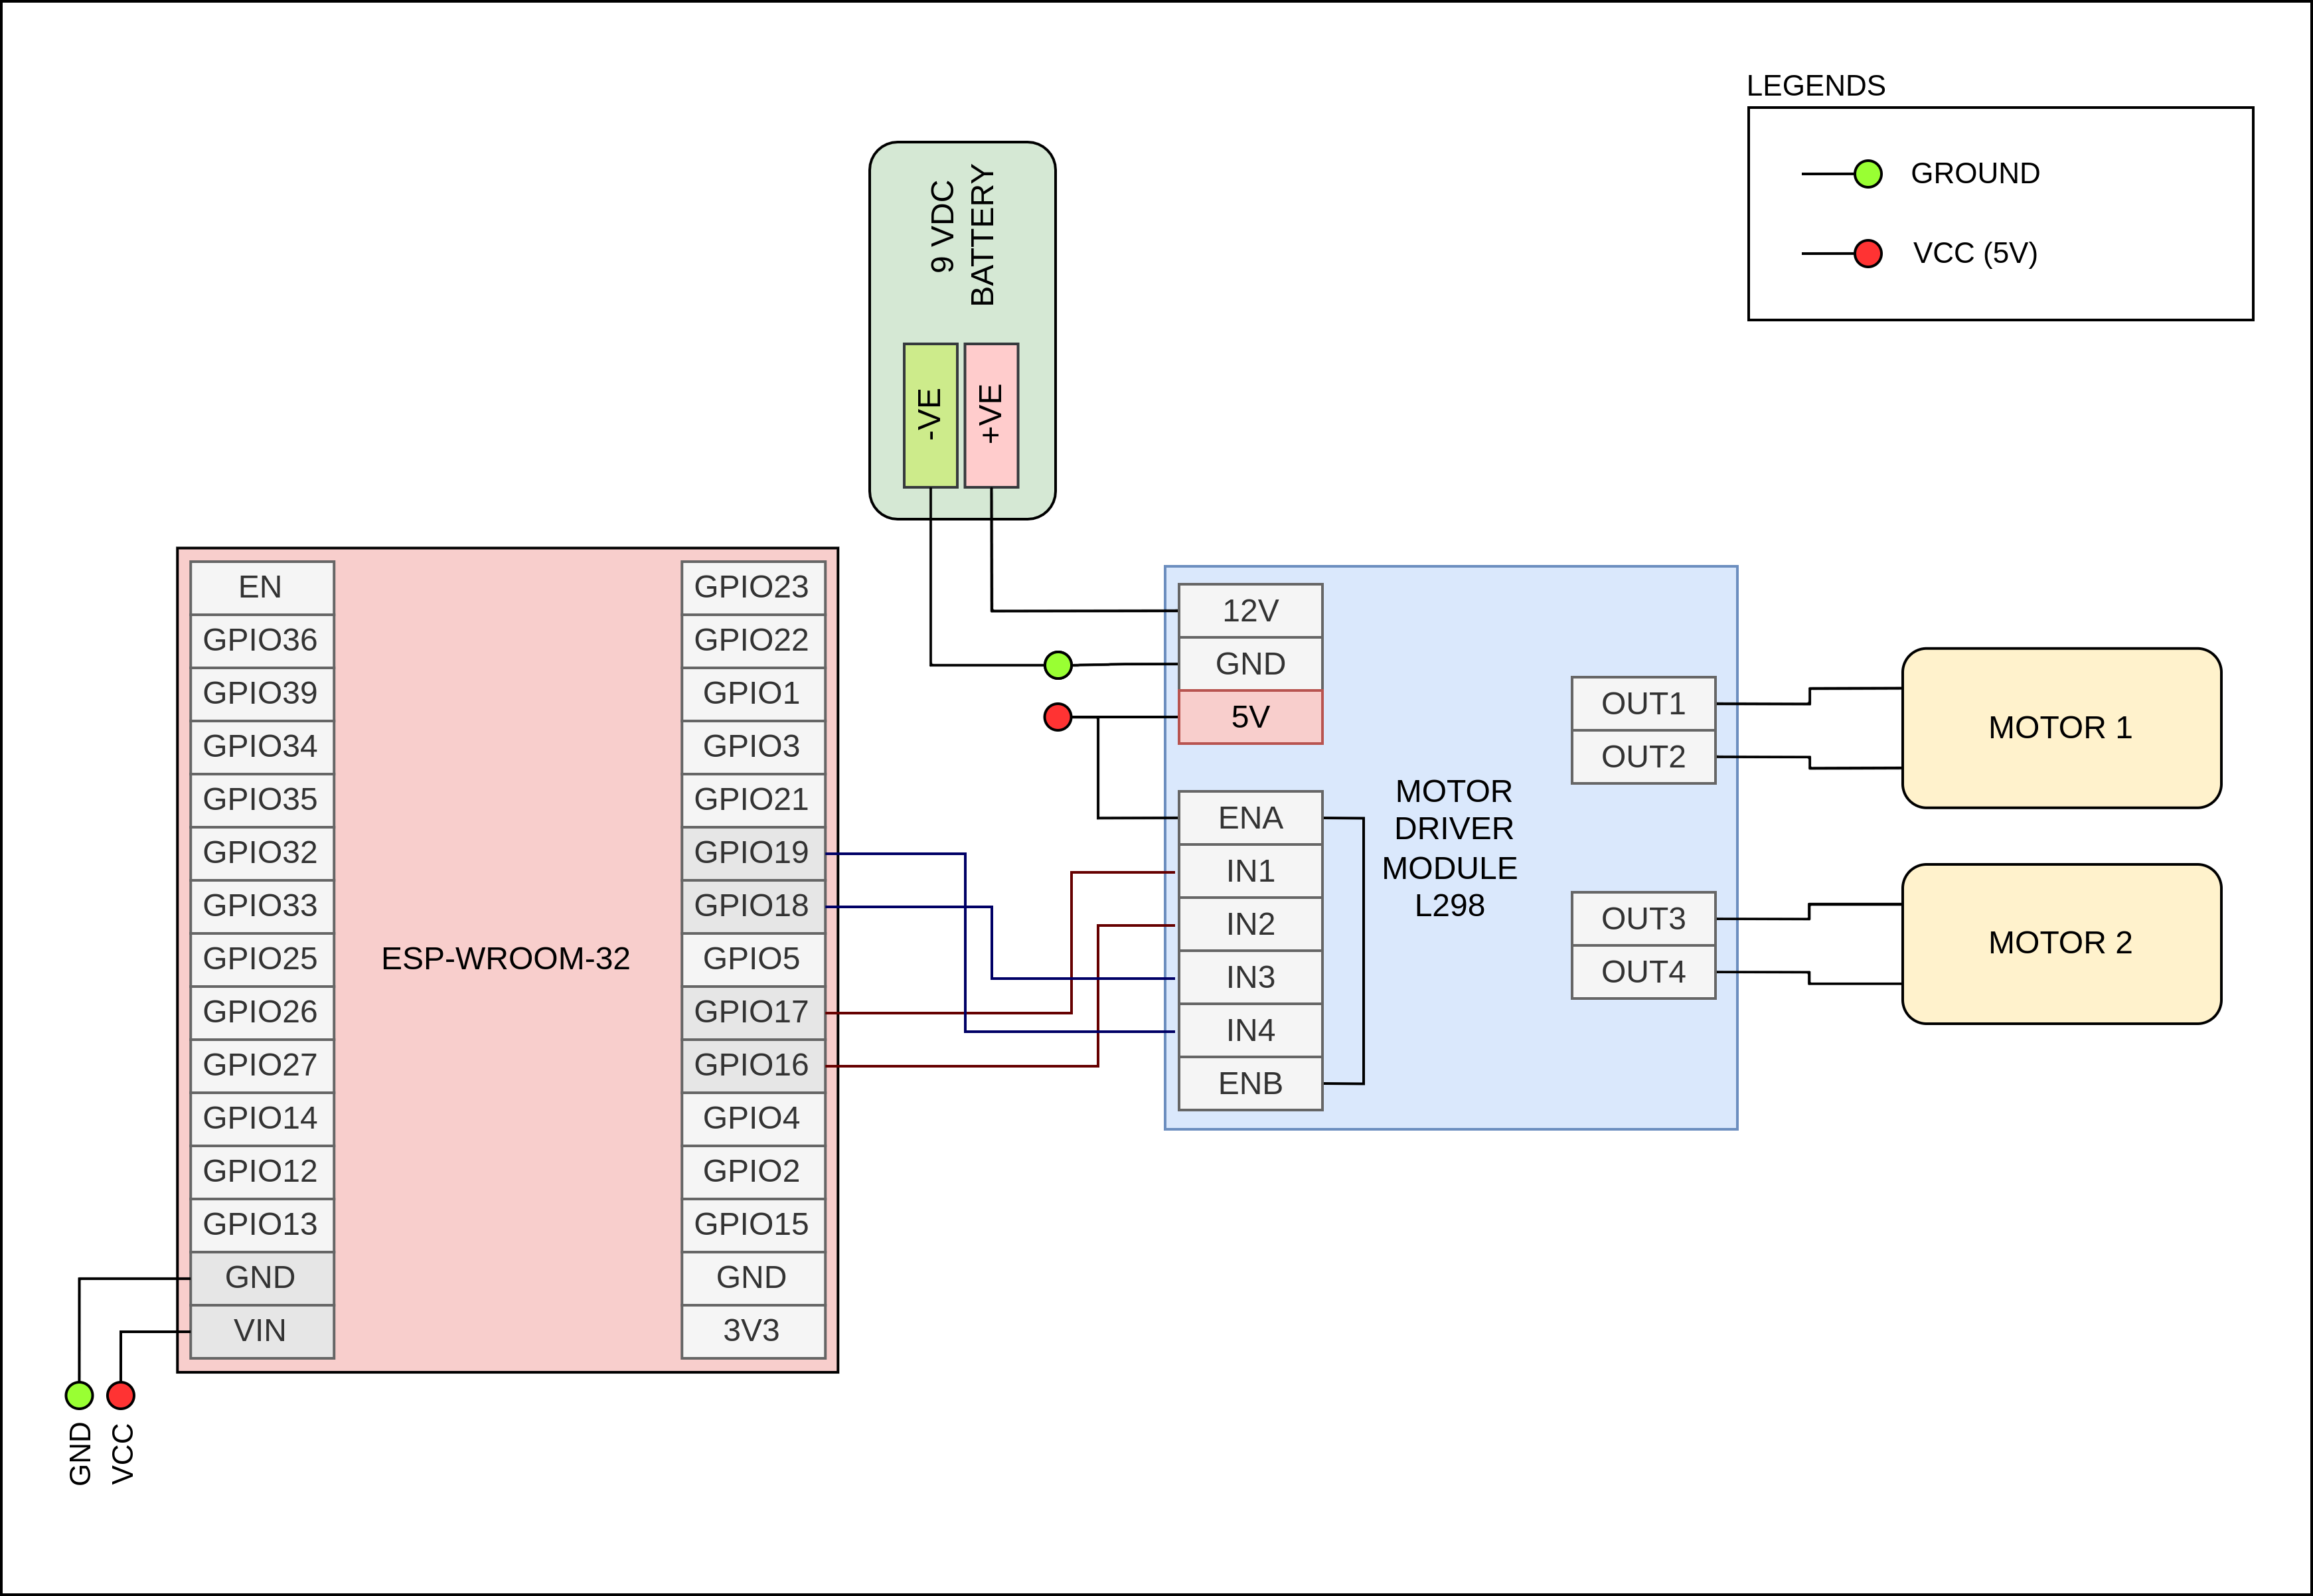
\includegraphics[width=\columnwidth]{./Figures/Wiring_UGV_speech.png}
\caption{Wiring Diagram for UGV Navigation using Speech commands}
\label{Wiring_UGV_speech}
\end{figure}

\begin{figure}[h!]
\centering
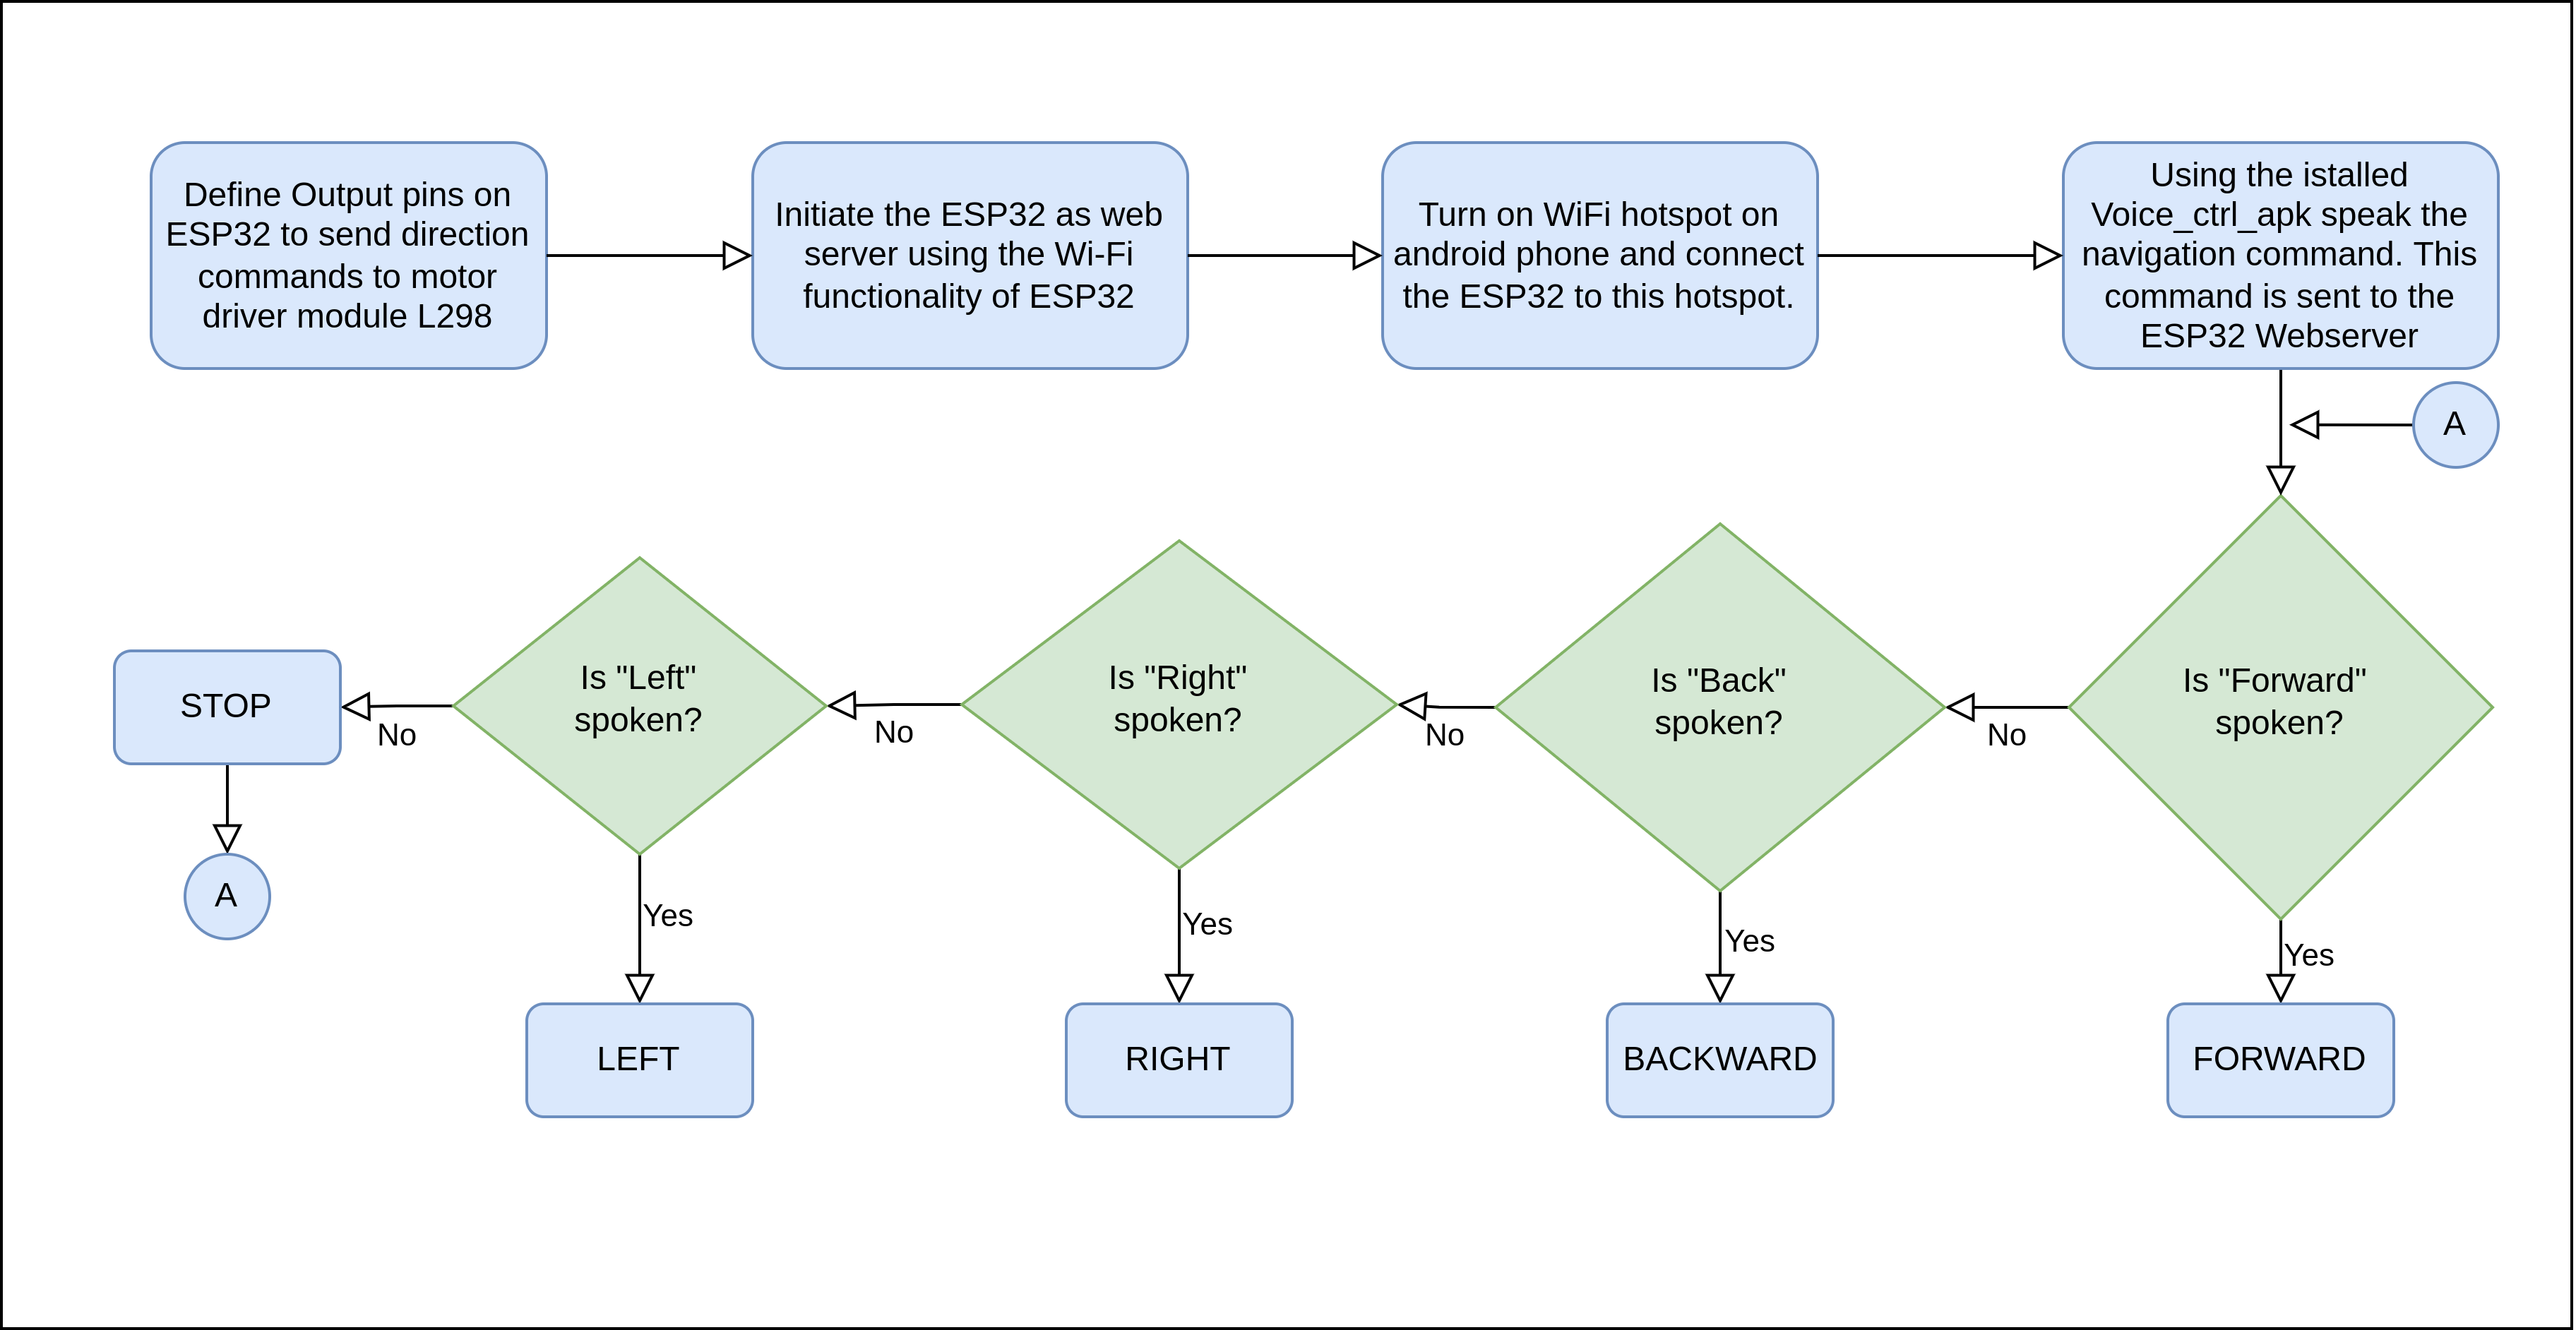
\includegraphics[width=\columnwidth]{./Figures/Flow_UGV_speech.png}
\caption{Flow Diagram for UGV Navigation using Speech commands}
\label{Flow_UGV_speech}
\end{figure}

\subsubsection{Code link} \label{Code_link_UGV_speech}
\begin{tcolorbox}
\url{https://github.com/sachinomdubey/Projects/tree/main/Autonomous\%20Navigation/UGV/ESP32/IDE/Voice_Controll_UGV}
\end{tcolorbox}



\subsubsection{Working}
\begin{itemize}
    \item User first speaks into the Speech\_ctrl\_IITH app (Figure \ref{Speech control app}) installed on android phone. The speech is converted to text using Google's TTS engine working at the background. 
    \item The text is sent over Wi-Fi connection to the ESP32 web server. 
    \item At ESP32, the program checks the command received and sends suitable commands (forward, backward, left, right and stop) to the direction control pins of Motor driver module L298N.
    \begin{figure}[H]
    \centering
    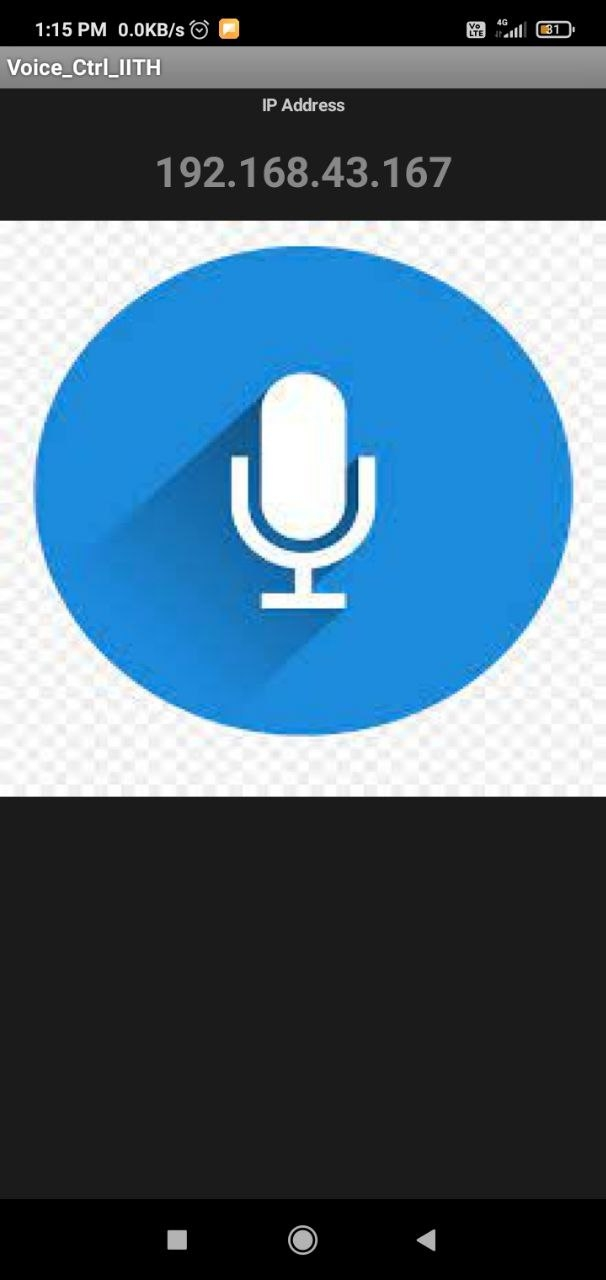
\includegraphics[width=5cm]{./Figures/Speech_ctrl_IITH.jpg}
    \caption{Speech control android app created using MIT app creator}
    \label{Speech control app}
    \end{figure}
\end{itemize}

\clearpage
\newpage
\subsection{Beacon Tracking using ESP32} 
\subsubsection{Required components/Software tools}
\begin{itemize}
    \item  UGV chassis with DC motors
    \item  ESP32 micro-controller with Type-B USB cable
    \item  L293D Motor Driver IC
    \item  Breadboard and Jumper Wires
    \item  Arduino IDE installed on system
    \item  Android phone used as beacon
\end{itemize}



\subsubsection{Steps}
\begin{itemize}
    \item Make the connections as per the wiring diagram (Figure \ref{Wiring_UGV_beacon}).
    \item Connect the ESP32 board to Laptop/PC using Type-B USB cable.
    \item Open the program at the code link (\ref{code_link_ESP32_beacon}) in Arduino IDE. From Tools menu, select suitable ”Board” and ”Port” for your ESP32 board.
    \item Compile the code by clicking on ”Verify” option. Upload the code to ESP32 using the ”Upload” option.
\end{itemize}

\subsubsection{{Code link}} \label{code_link_ESP32_beacon}
\begin{tcolorbox}
\url{https://github.com/sachinomdubey/Projects/tree/main/Autonomous\%20Navigation/UGV/ESP32/IDE/Beacon_tracking}
\end{tcolorbox}

\begin{figure}[h!]
\centering
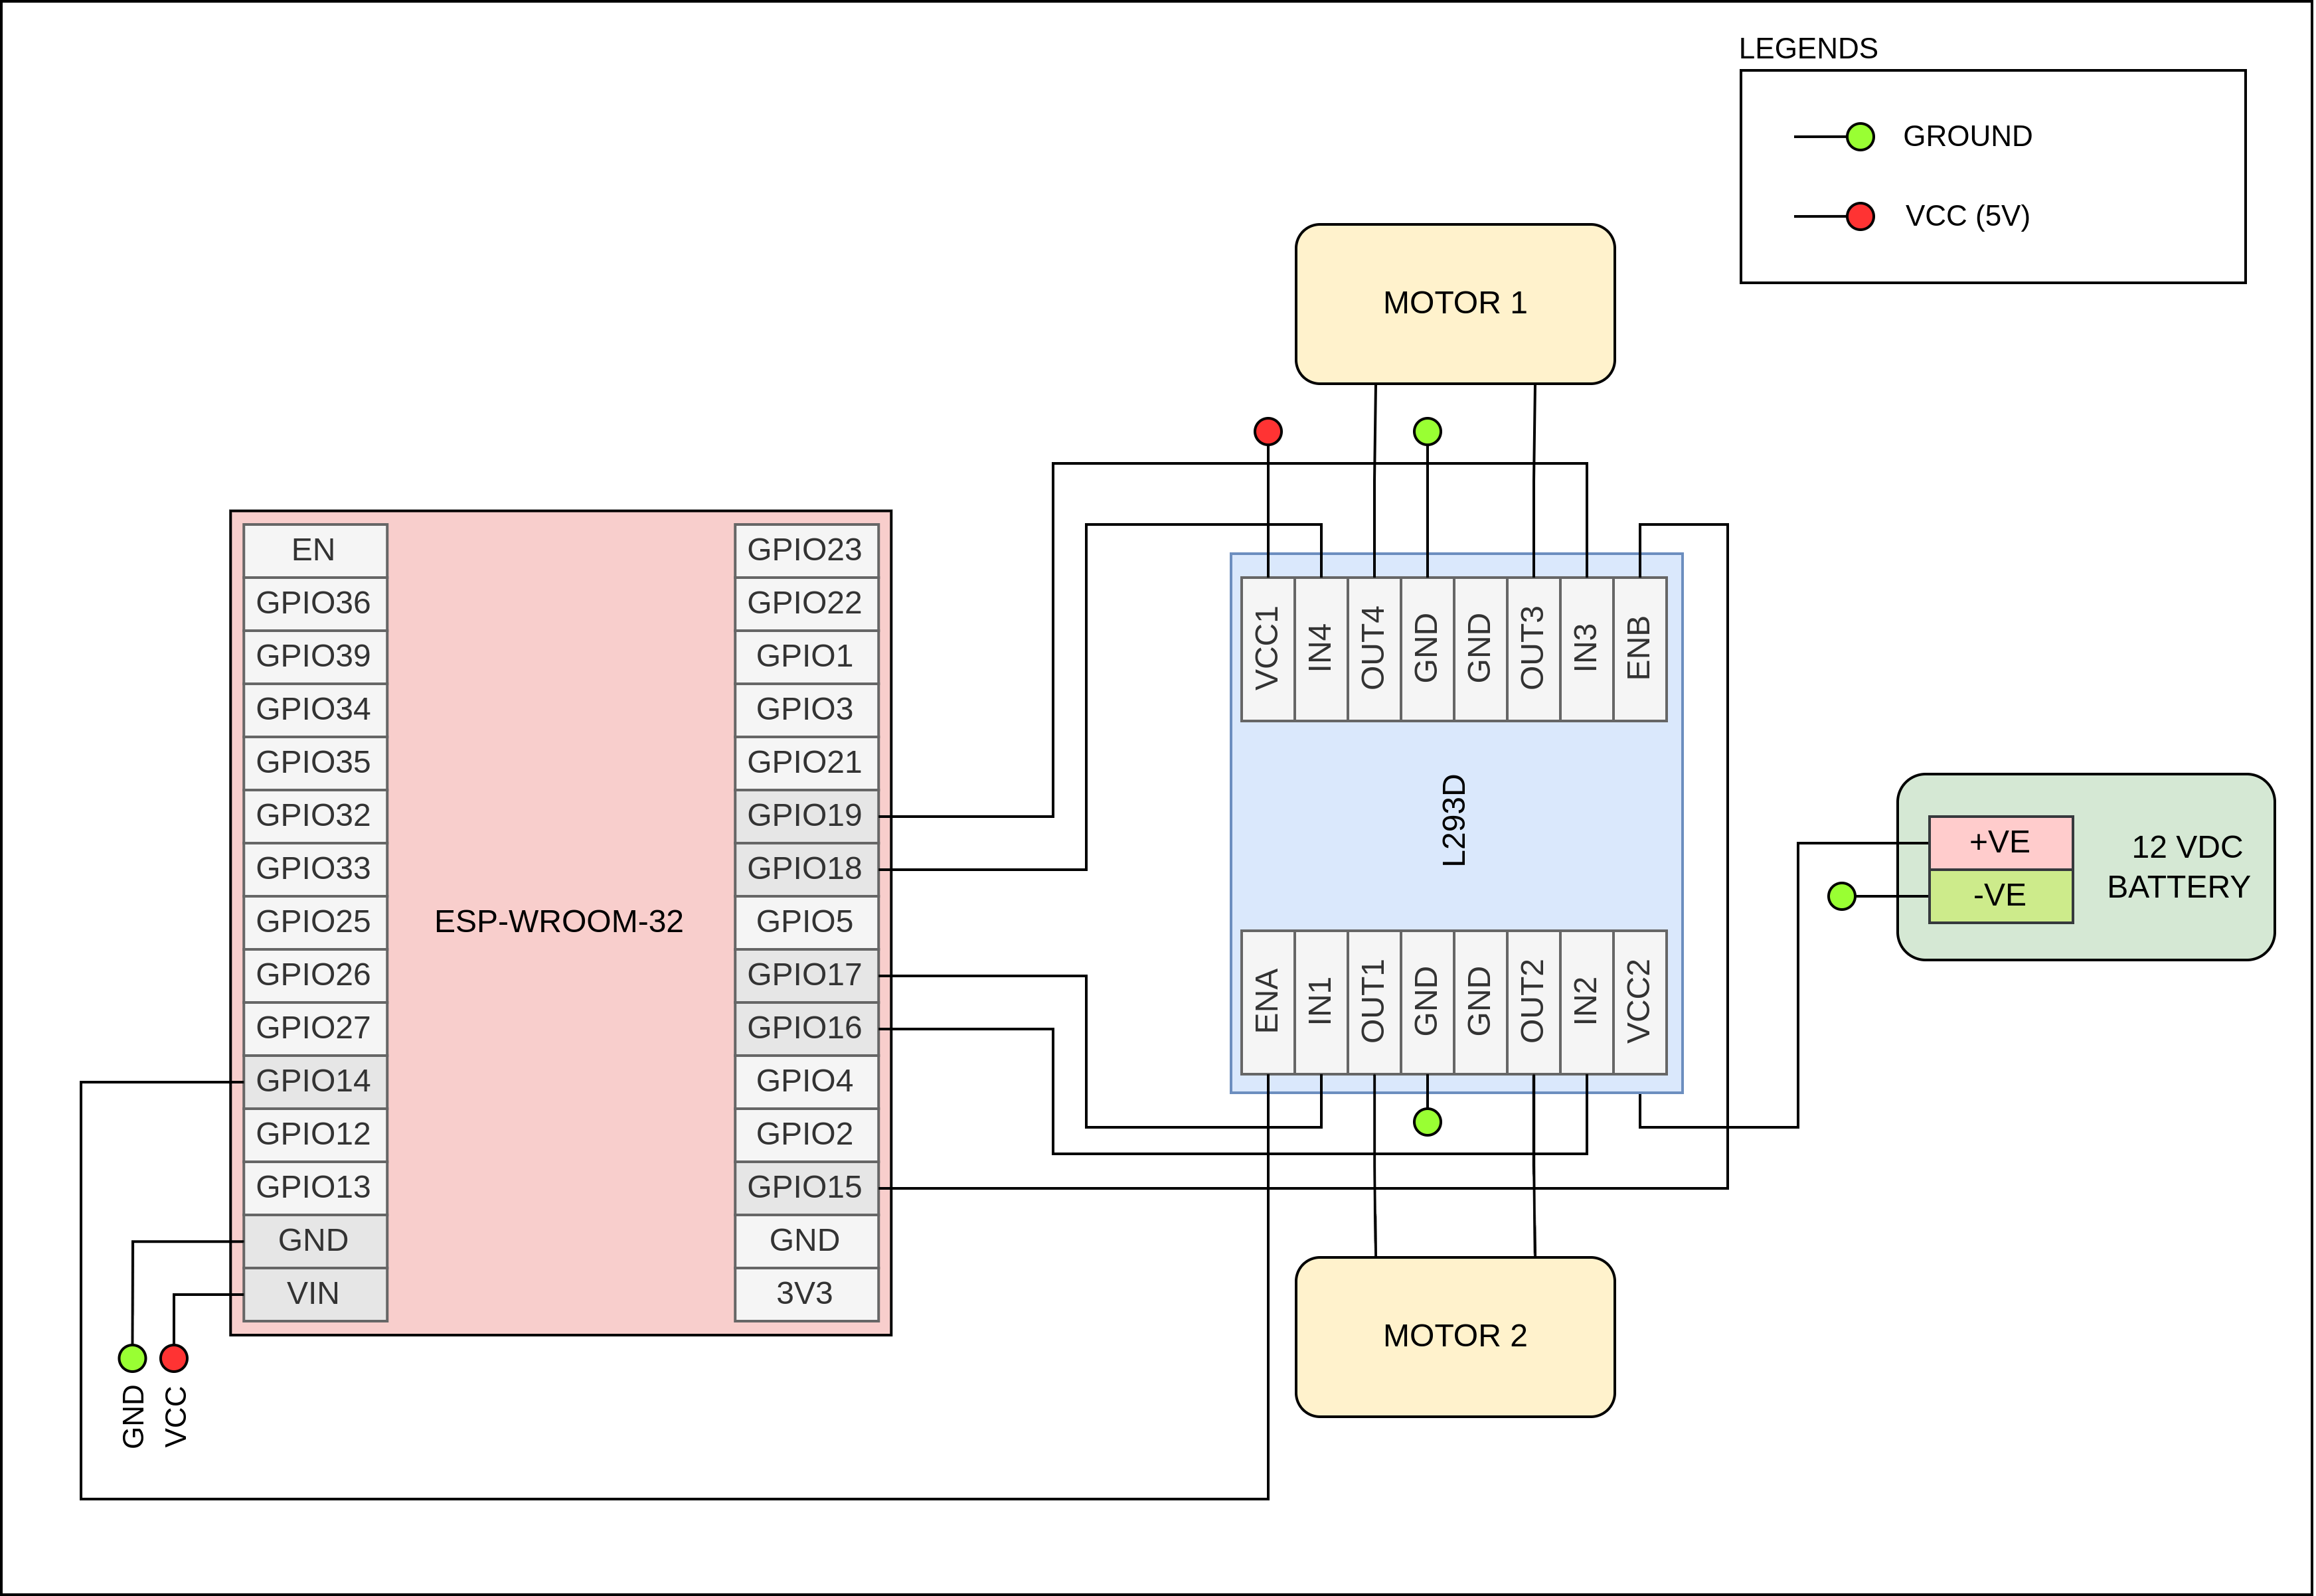
\includegraphics[width=\columnwidth]{./Figures/Wiring_UGV_beacon.png}
\caption{Wiring Diagram for UGV beacon tracking}
\label{Wiring_UGV_beacon}
\end{figure}

\begin{figure}[h!]
\centering
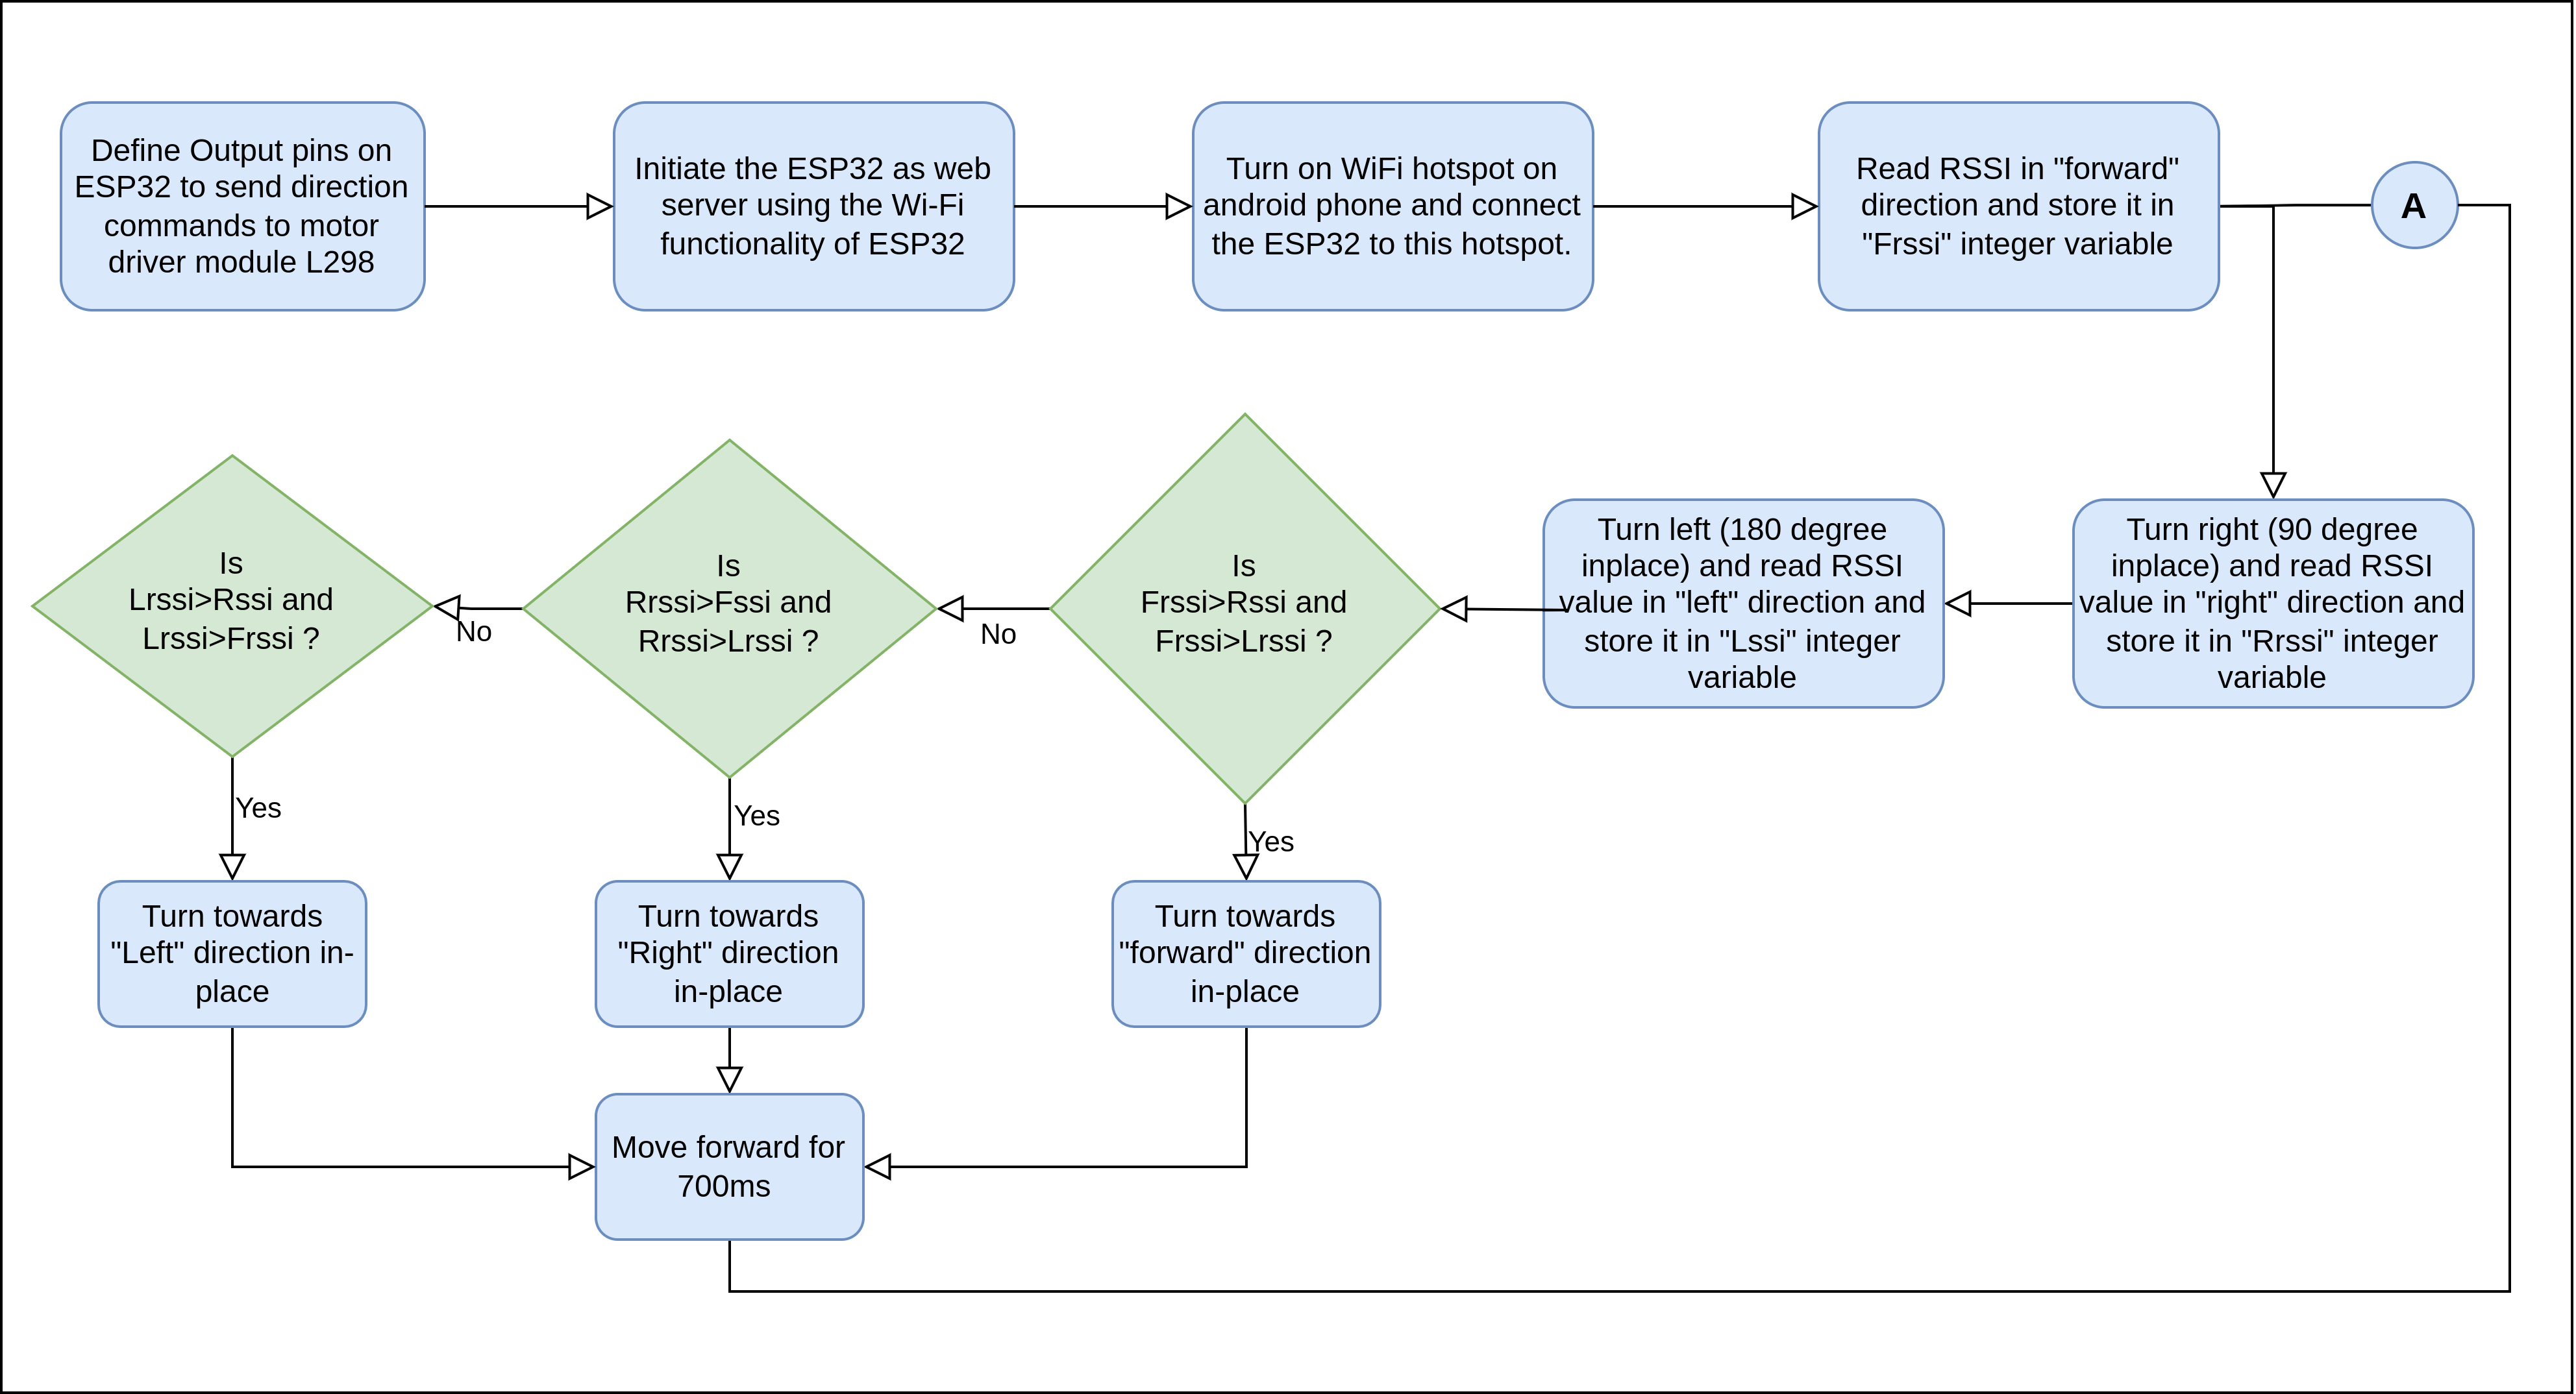
\includegraphics[width=\columnwidth]{./Figures/Flow_UGV_beacon.png}
\caption{Flow Diagram for UGV beacon tracking}
\label{Flow_UGV_beacon}
\end{figure}

\subsubsection{Working}
\begin{itemize}
    \item Initially, ESP32 mounted on the car will read RSSI (Radio Signal Strength Indicator) levels in forward, right and left direction by suitable in-place rotation.
    \item Average of 20 RSSI values are taken while measuring RSSI level in a particular direction. This is done in order to read stable RSSI
    values.
    \item The car then rotates towards the direction having the highest RSSI level.
    \item Further, It moves forward for a certain distance towards the beacon. By repeating above steps again and again, the car navigates towards the beacon.
\end{itemize}

\section{UAV (Unmanned Aerial Vehicle)}
\subsection{Navigation using ESP32 and Android phone} 
\subsubsection{Required components/Software tools}
\begin{itemize}
    \item UAV fully assembled and configured.
    \item ESP32 micro-controller with Type-B USB cable for programming.
    \item Jumper Wires
    \item Arduino IDE installed on system
    \item Android phone with chrome web browser to access ESP32 web-server.
\end{itemize}

\subsubsection{Steps}
\begin{itemize}
    \item Make the connections as per the wiring diagram (Figure \ref{Wiring_UAV_ESP32_commlink}).
    \item Go to Arduino IDE and write the following program available on the code link at \ref{Code_link_UAV_ESP32_commlink}.
    \item Compile and upload the program to ESP32 micro-controller using the Type-C programmable cable. 
    \item Arm the drone using Yaw and Throttle slider and slowly increase the throttle slider to lift the drone vertically from the ground.
    \item Try navigation the UAV using the various sliders (Throttle, Yaw, Roll, pitch) on the Android phone.
\end{itemize}

\subsubsection{Code link} \label{Code_link_UAV_ESP32_commlink}
\begin{tcolorbox}
\url{https://github.com/sachinomdubey/Projects/blob/main/Autonomous\%20Navigation/UAV/ESP32_comm_link/pwmwebserver_esp32}
\end{tcolorbox}

\begin{figure}[h!]
\centering
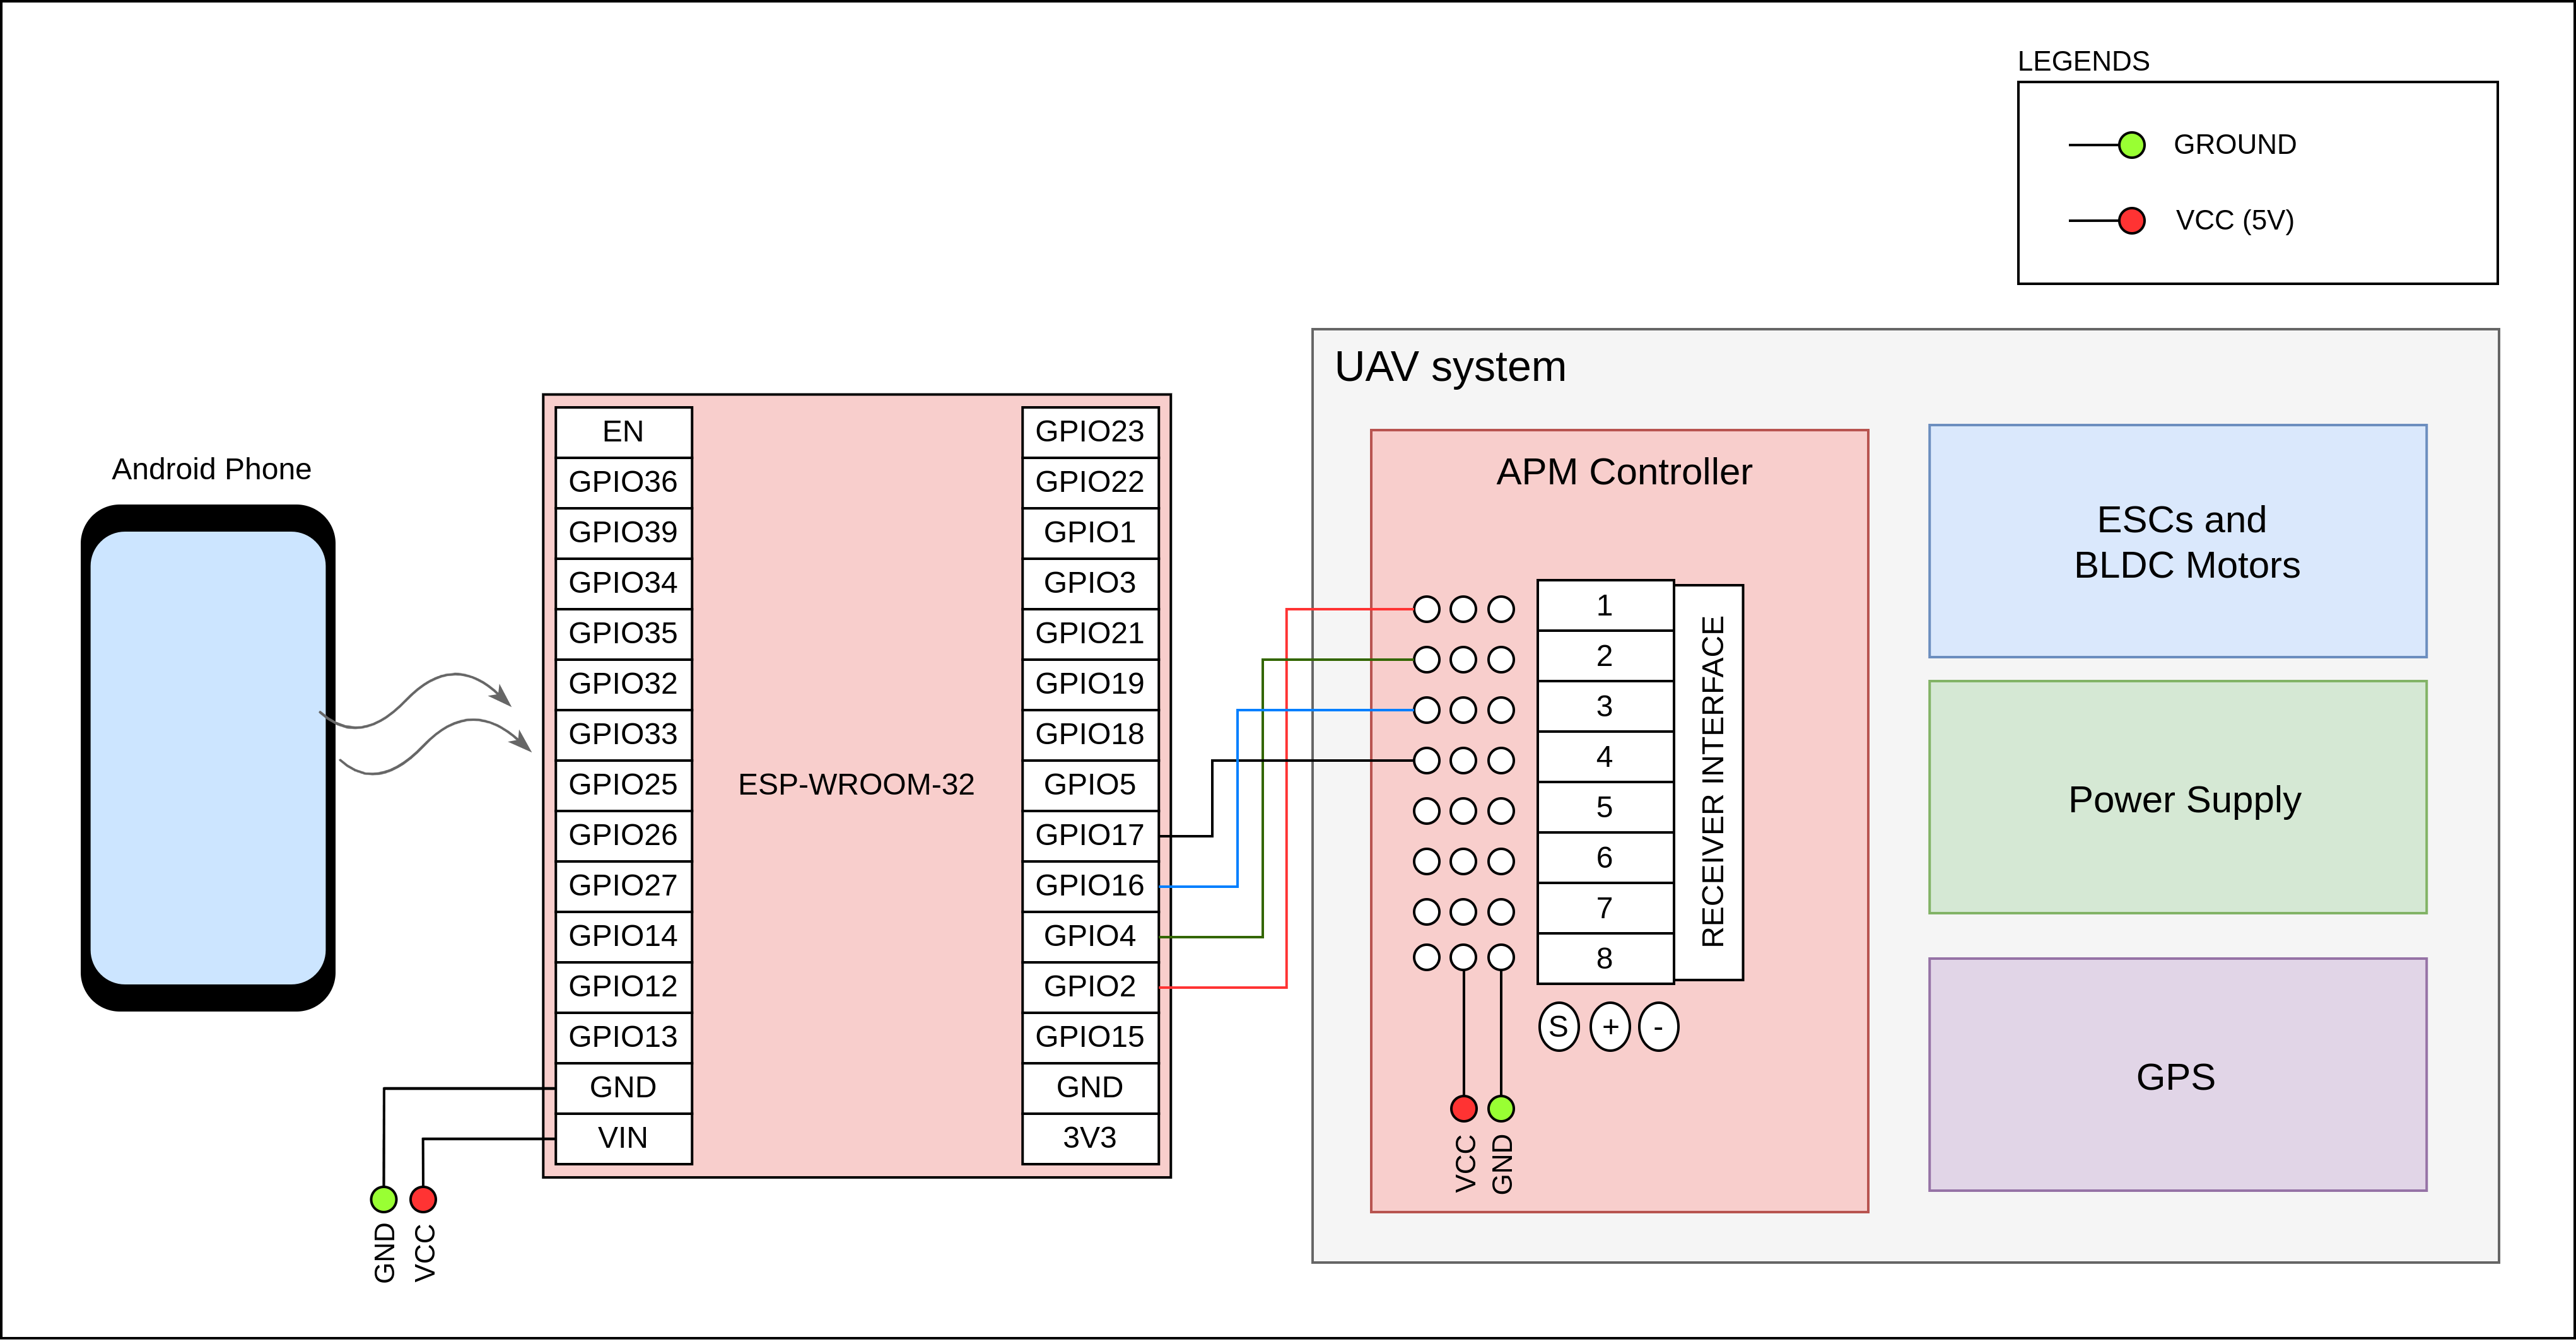
\includegraphics[width=\columnwidth]{./Figures/Wiring_UAV_ESP32_commlink.png}
\caption{Wiring Diagram for UAV Navigation using ESP32 and Android phone}
\label{Wiring_UAV_ESP32_commlink}
\end{figure}

\begin{figure}[ht]
\centering
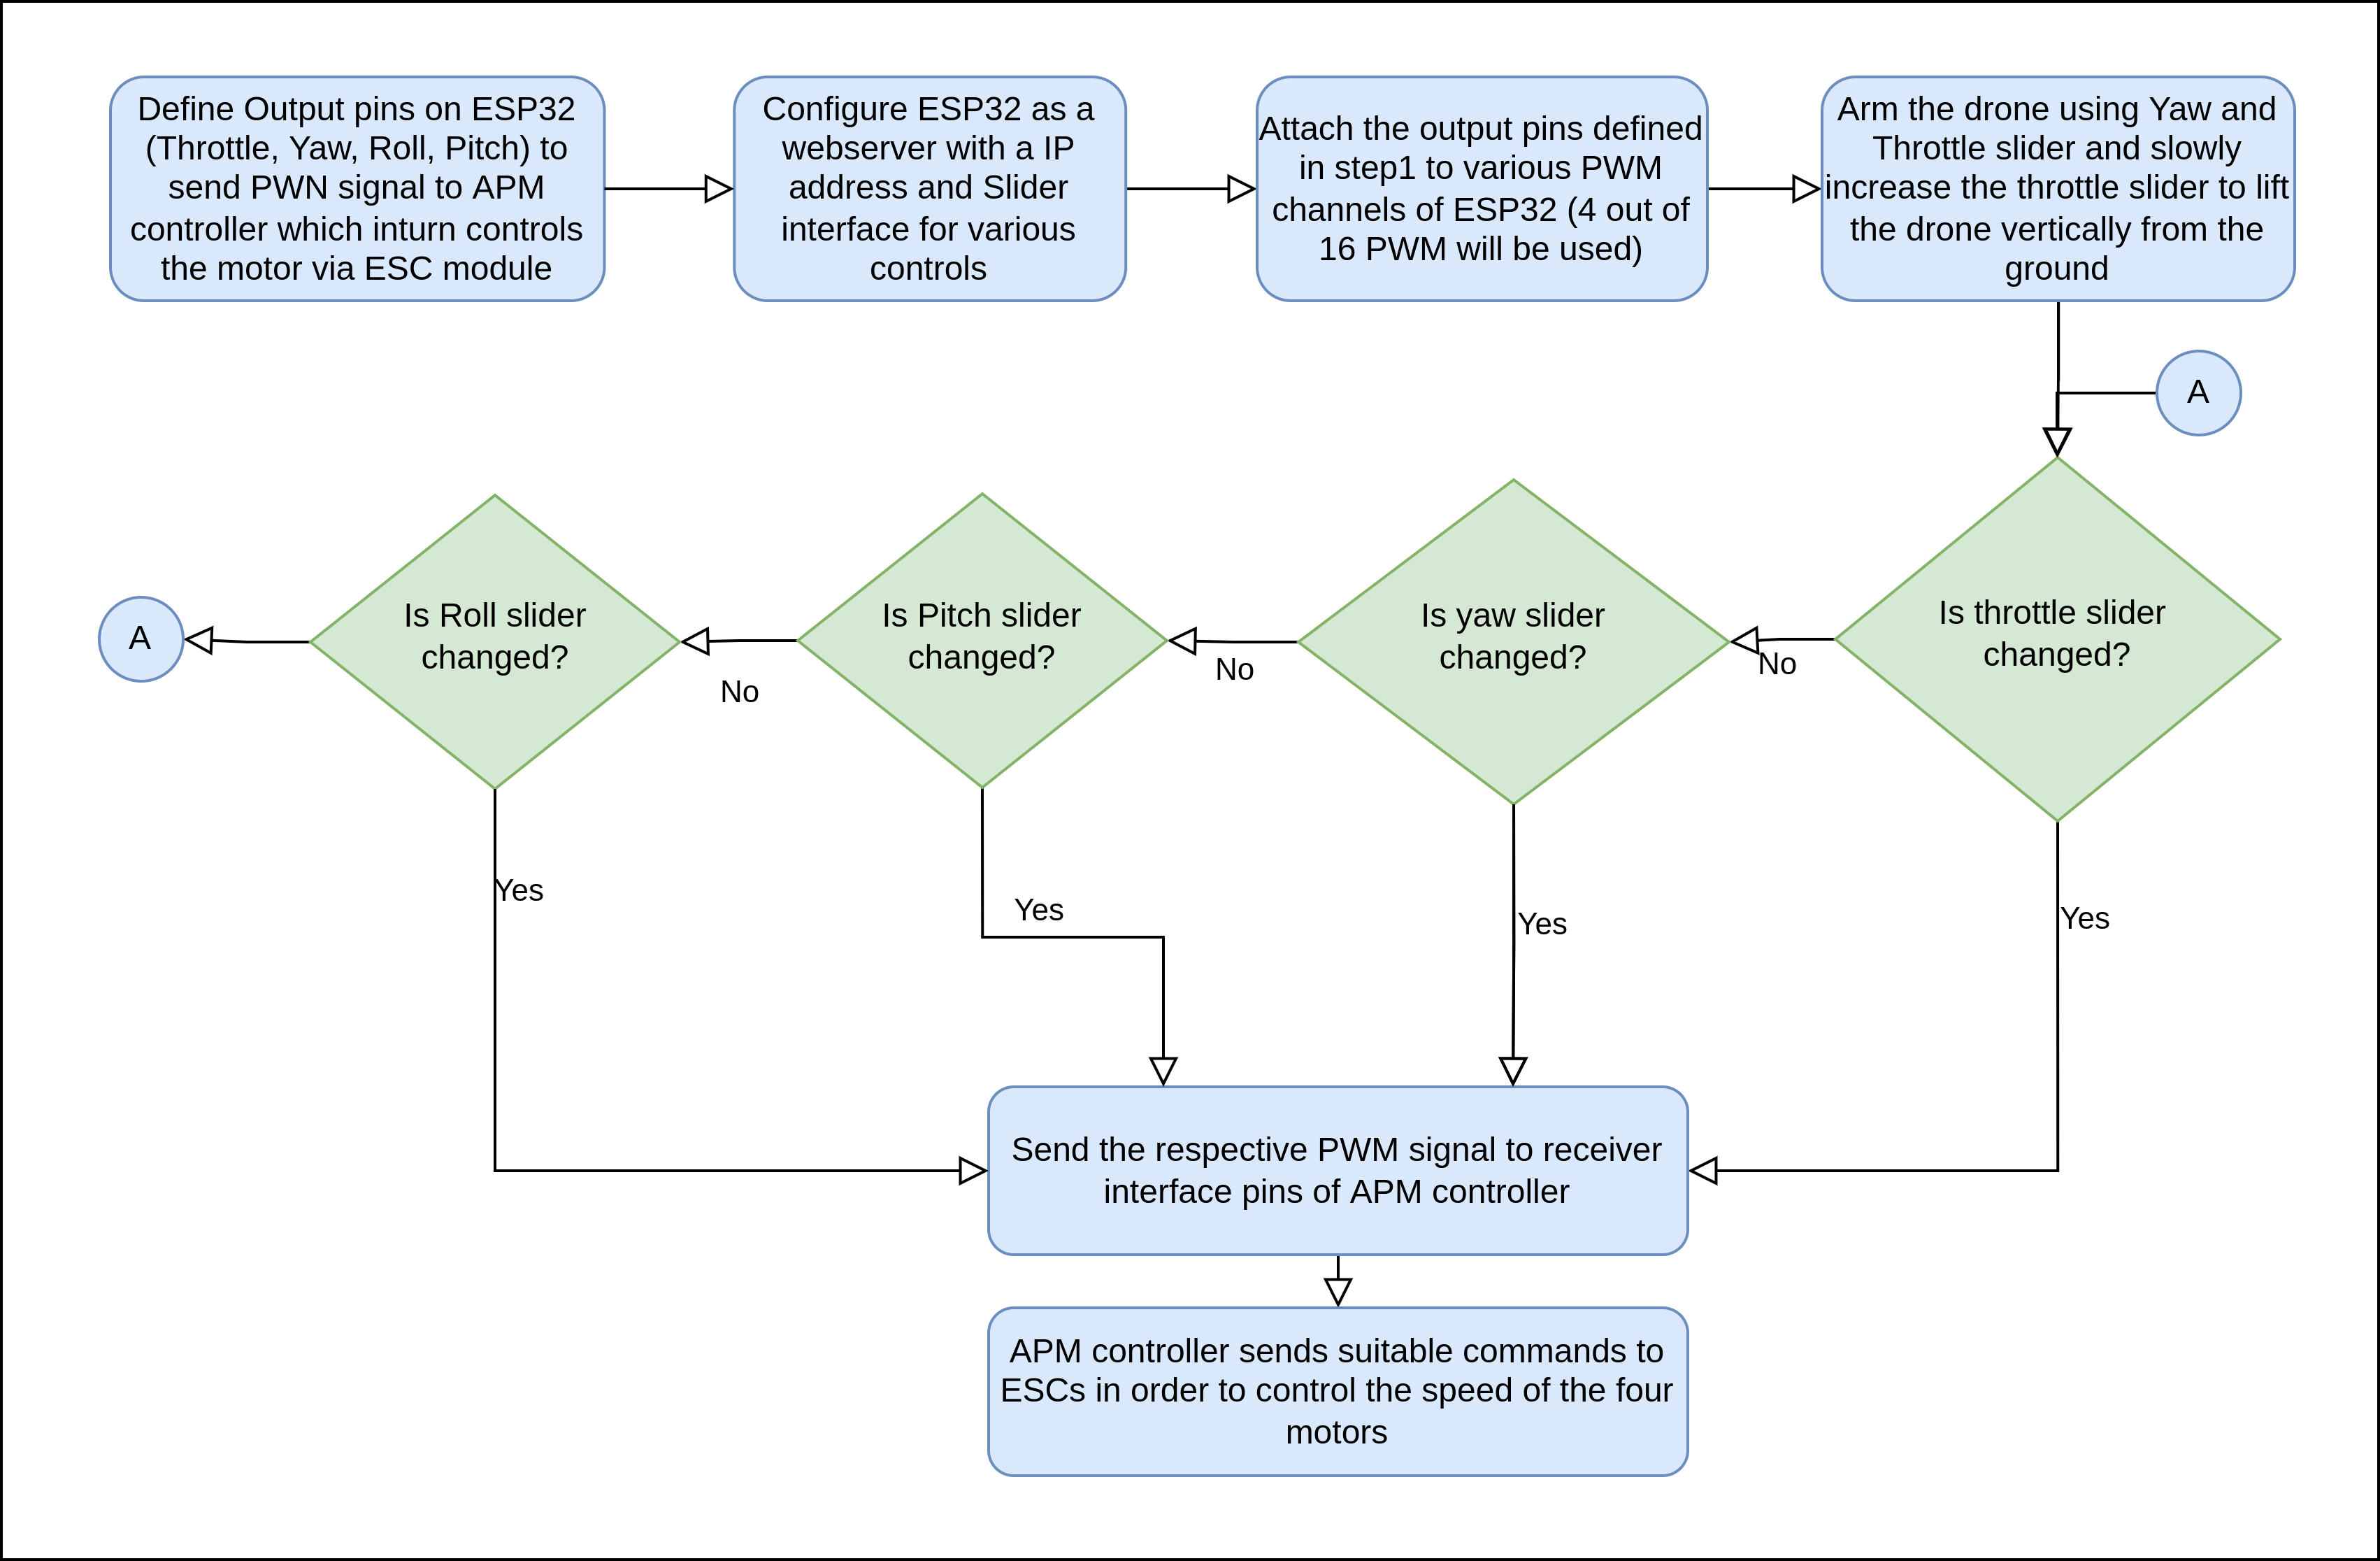
\includegraphics[width=14cm]{./Figures/Flow_UAV_ESP32_commlink.png}
\caption{Flow Diagram for UAV Navigation using ESP32 and Android phone}
\label{Flow_UAV_ESP32_commlink}
\end{figure}

\newpage
\subsubsection{Working}
\begin{itemize}
    \item User first arms the drone using Yaw and Throttle slider (analogous to arming using fly-sky transmitter) and slowly increase the throttle slider to lift the drone vertically from the ground.
    \item Whenever a slider is changed by user the ESP32 reads this change and generates a PWM signal (same as generated by the Fly-sky receiver module).
    \item Depending on the duty-cycle of this signal the APM controller drives the four ESC modules which further controls the speech of the four BLDC motors. (Refer section \ref{Basics_motor_control} for details on control of speed of BLDC motors)
    \item Thus, the Android phone and ESP32 form a new communication link from ground operator to drone controller. The range of this link is limited by the Wi-Fi network to which the ESP32 and android phones are connected.
\end{itemize}

\newpage

\section{Running two tasks simultaneously using FreeRTOS (Arduino) }
Embedded systems uses real-time operating system. Real-time tasks are critical as timing places an important role in such systems. RTOS are made to run tasks or program with precise timings and high degree of reliability. It helps in multitasking even when the micro-controller unit has a single core to execute these tasks.

FreeRTOS is an open source RTOS which are designed, but not limited to run on small micro-controllers (8/16 bit). With basic knowledge of RTOS, we can use FreeRTOS as there is a lot of documentation available for it.

In this program, we have run two different tasks in parallel on Arduino Uno using FreeRTOS. The two tasks are as follow:
\begin{enumerate}
    \item Blinking LED connected at pin 13 of Arduino.
    \item Speeding up and slowing down a DC motor continuously in a loop.
\end{enumerate}

\subsubsection{Required components/Software tools}
\begin{itemize}
    \item Arduino Uno R3 board
    \item LED connected between pin 13 and GND.
    \item L293D motor driver IC
    \item 12V DC Battery for motor
    \item Type-B cable for powering Arduino
    \item Jumper Wires
    \item Arduino IDE installed on system
\end{itemize}

\begin{figure}[ht]
\centering
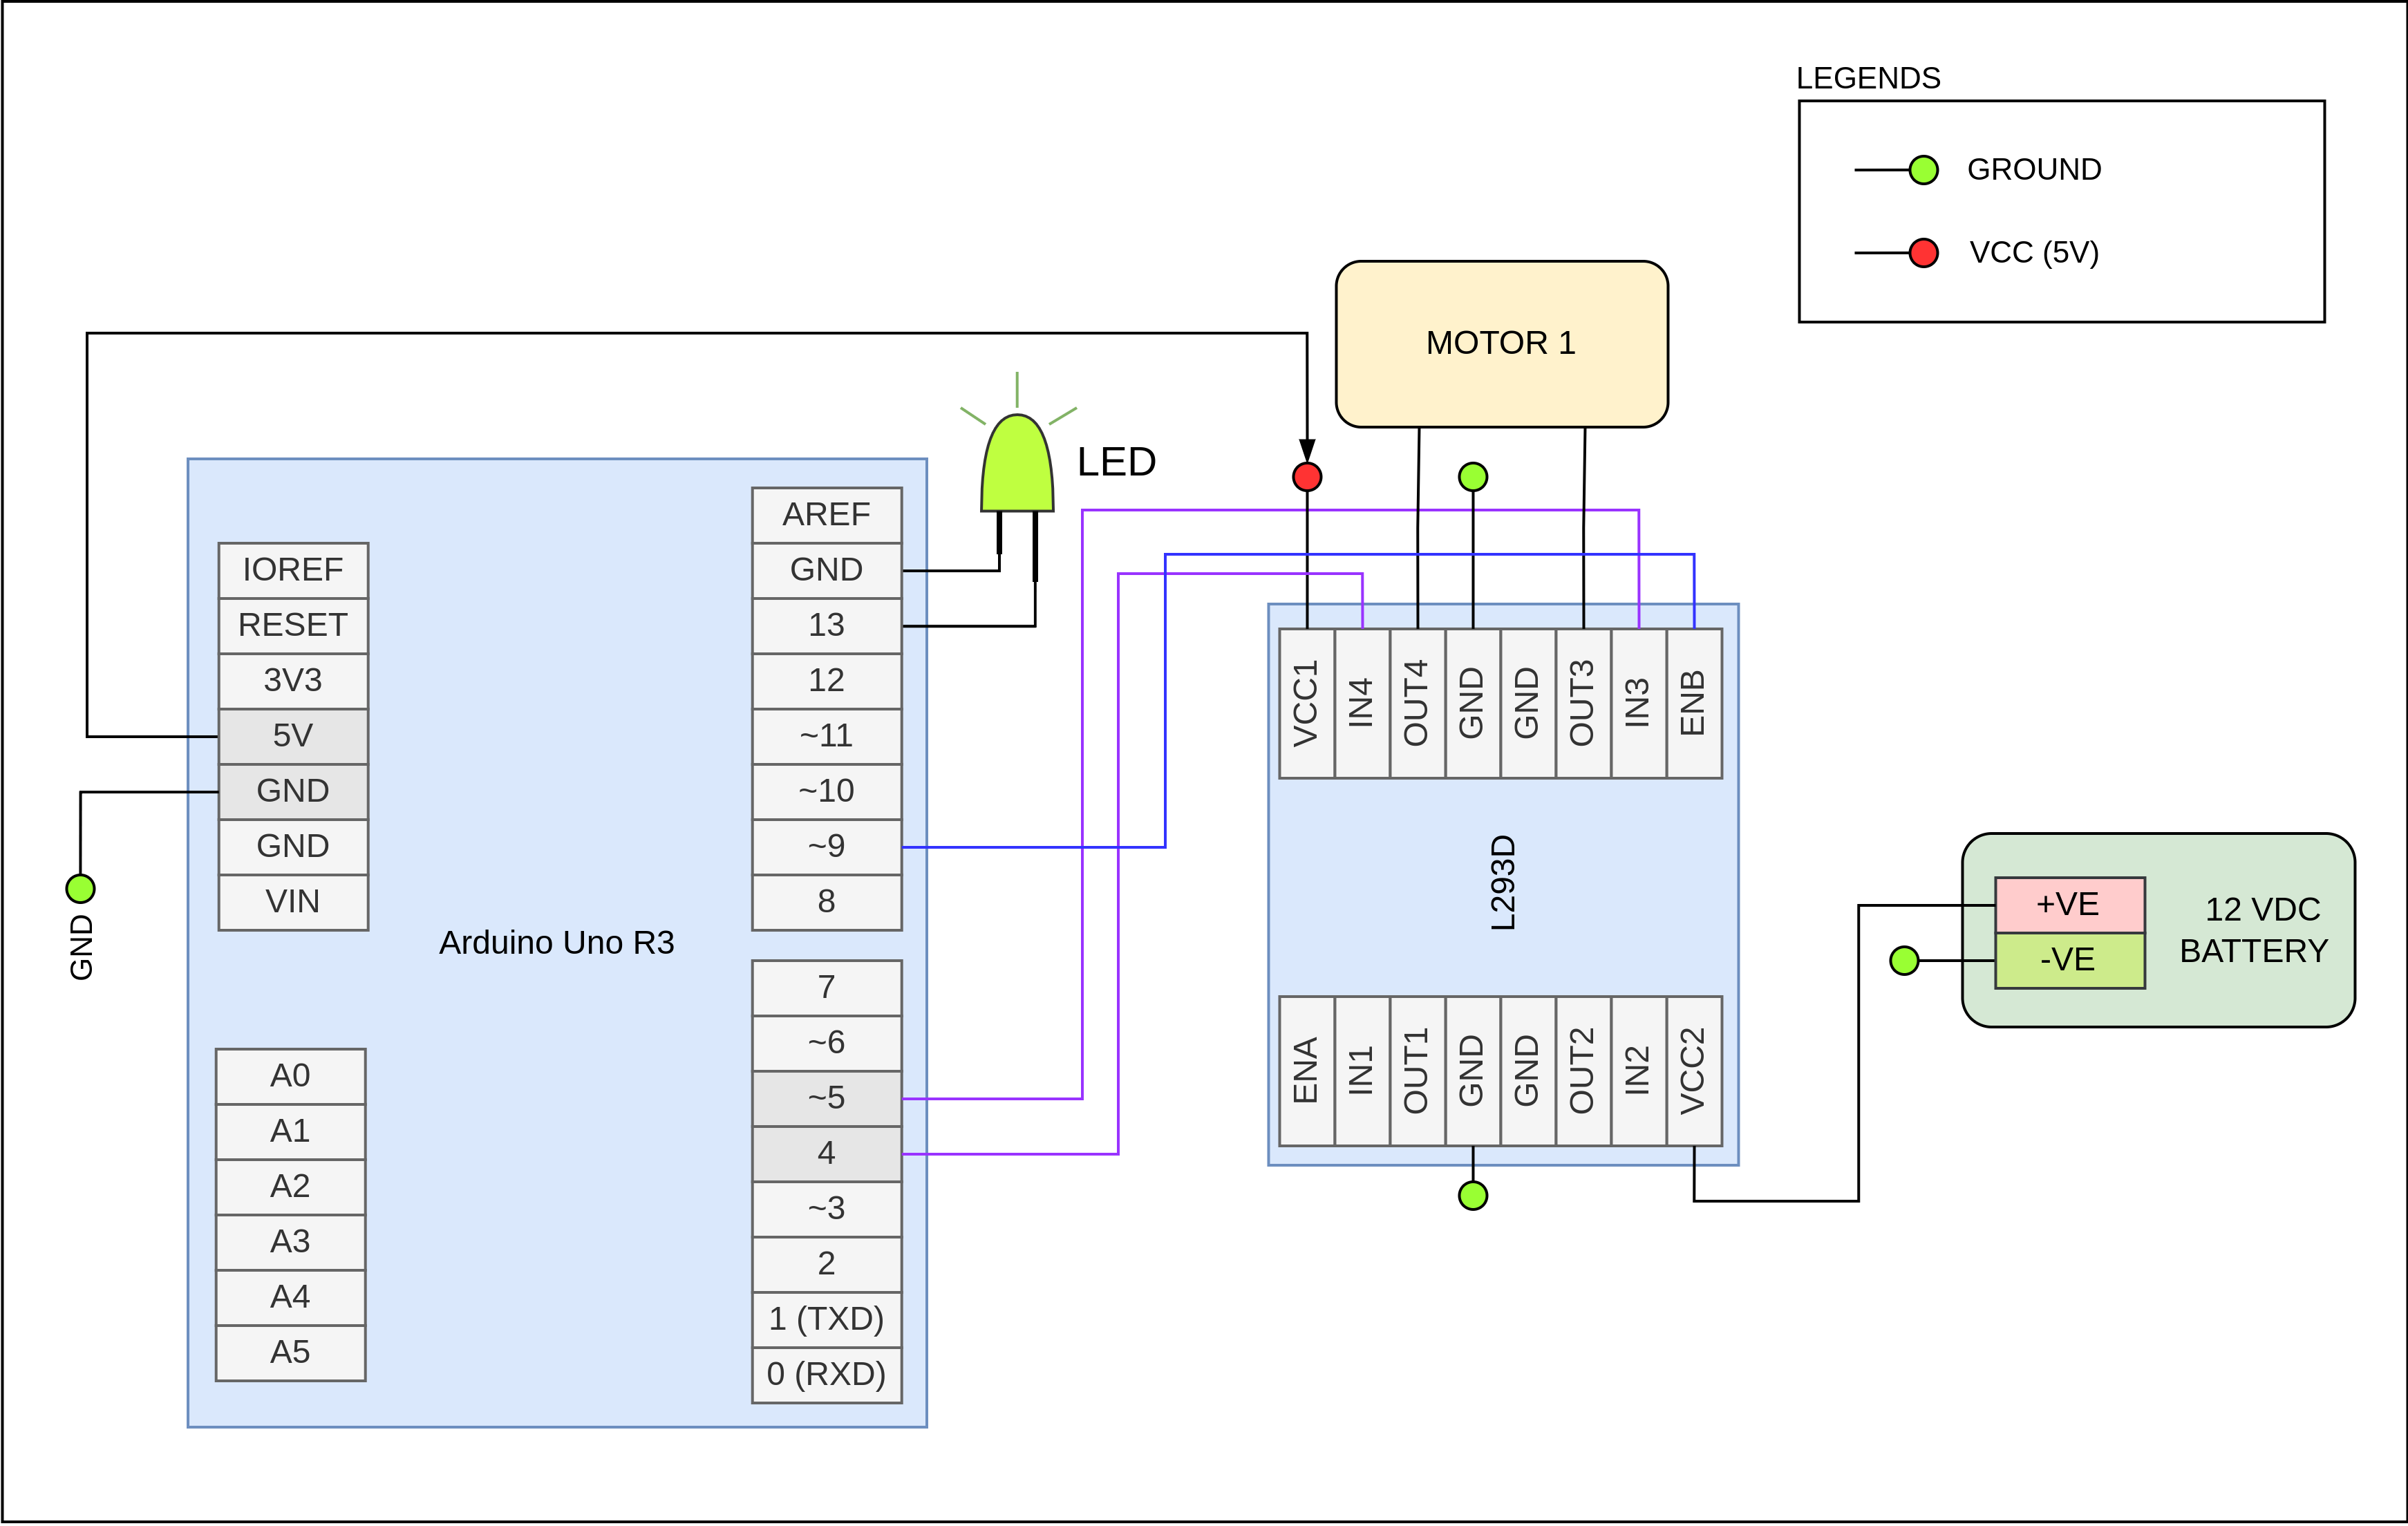
\includegraphics[width=\columnwidth]{./Figures/Wiring_FreeRTOS_demo.png}
\caption{Wiring diagram for running two tasks simultaneously on Arduino Uno.}
\label{Wiring_FreeRTOS_demo}
\end{figure}

\subsubsection{Steps}
\begin{itemize}
    \item Make the connections as per the wiring diagram (Figure \ref{Wiring_FreeRTOS_demo}).
    \item Connect the Arduino Uno to Laptop/PC using Type-B USB cable.
    \item Open the program at the code link (\ref{Code_link_FreeRTOS_Arduino}) in Arduino IDE.
    \item From Tools menu, select suitable ”Board” and ”Port” for your Arduino board.
    \item Compile the code by clicking on ”Verify” option.
    \item Upload the code to ESP32 using the ”Upload” option.
    \item Verify that the LED blinks and the motor also changes speed simultaneously.
\end{itemize}

\subsubsection{Code link} \label{Code_link_FreeRTOS_Arduino}
\begin{tcolorbox}
\url{https://github.com/sachinomdubey/Projects/tree/main/Autonomous\%20Navigation/FreeRTOS/Arduino_Blink_MotorControl/Code}
\end{tcolorbox}

\subsubsection{Working}
\begin{itemize}
    \item First the FreeRTOS library is included using the below line. This header contains all the functions required to create, schedule and run tasks in parallel.
    \begin{lstlisting}[language=C]
    #include <Arduino_FreeRTOS.h>
    \end{lstlisting}
    \item For creating task, \textbf{xTaskCreate()} API is called in setup function with certain parameters/arguments.
    \begin{lstlisting}[language=C]
    xTaskCreate( TaskFunction_t pvTaskCode, const char * const pcName,
    uint16_t usStackDepth, void *pvParameters, UBaseType_t uxPriority,
    TaskHandle_t *pxCreatedTask );
    \end{lstlisting}
    \item There are 6 arguments that should be passed while creating any task. Let’s see what these arguments are ~\cite{FreeRTOS_task}:
    \begin{itemize}
        \item \textbf{pvTaskCode}: It is simply a pointer to the function that implements the task (in effect, just the name of the function).
        \item \textbf{pcName}: A descriptive name for the task. This is not used by FreeRTOS. It is included purely for debugging purposes.
        \item \textbf{usStackDepth}: Each task has its own unique stack that is allocated by the kernel to the task when the task is created. The value specifies the number of words the stack can hold, not the number of bytes. For example, if the stack is 32-bits wide and usStackDepth is passed in as 100, then 400 bytes of stack space will be allocated (100 * 4 bytes) in RAM. Use this wisely because Arduino Uno has only 2Kbytes of RAM.
        \item \textbf{pvParameters}: Task input parameter (can be NULL).
        \item \textbf{uxPriority}: Priority of the task ( 0 is the lowest priority).
        \item \textbf{pxCreatedTask}: It can be used to pass out a handle to the task being created. This handle can then be used to reference the task in API calls that, for example, change the task priority or delete the task (can be NULL).
    \end{itemize}
    \item Example of task creation
    \begin{lstlisting}
    xTaskCreate(task1,"task1",128,NULL,1,NULL);
    xTaskCreate(task2,"task2",128,NULL,2,NULL);  
    \end{lstlisting}
    \item After creating the task, start the scheduler in a void setup using \textbf{vTaskStartScheduler()} API.
    \item \textbf{Void loop()} function will remain empty as we don’t want to run any task manually and infinitely. Because task execution is now handled by Scheduler.
    \item Next we define our tasks using below format and write logic for it. Everything else is taken by FreeRTOS library function and we can observe the tasks running in parallel on executing the written program.
    \begin{lstlisting}
    void task1(void *pvParameters)  
    {
        while(1) {
            ..
            ..//your logic
        }
    }
    \end{lstlisting}
\end{itemize}







